\documentclass[article,type=msc,colorback,accentcolor=tud9c,twoside,11pt]{tudthesis}
\usepackage{titlesec}

%\usepackage{german}
\usepackage{amsmath}
\usepackage{algorithm}
\usepackage{tocloft}
\usepackage{chngcntr}
\counterwithin{figure}{section}
\usepackage[normalem]{ulem}
\usepackage{wrapfig}
\usepackage{amsmath}
\usepackage{algpseudocode}
%\usepackage[ansinew]{inputenc}
\newcommand{\getmydate}{%
	\ifcase\month%
	\or Januar\or Februar\or M\"arz%
	\or April\or Mai\or Juni\or Juli%
	\or August\or September\or Oktober%
	\or November\or Dezember%
	\fi\ \number\year%
}    
\usepackage{hyperref}
\usepackage{multirow}
\usepackage{float}
\usepackage{caption}
\usepackage[ngerman,english]{babel}
\usepackage{listings}
\usepackage{color}
\definecolor{dkgreen}{rgb}{0,0.6,0}
\definecolor{gray}{rgb}{0.5,0.5,0.5}
\definecolor{mauve}{rgb}{0.58,0,0.82}

\lstset{frame=tb,
	language=Java,
	aboveskip=3mm,
	belowskip=3mm,
	showstringspaces=false,
	columns=flexible,
	basicstyle={\small\ttfamily},
	numbers=none,
	numberstyle=\tiny\color{gray},
	keywordstyle=\color{blue},
	commentstyle=\color{dkgreen},
	stringstyle=\color{mauve},
	breaklines=true,
	breakatwhitespace=true,
	tabsize=3
}
\usepackage{tikz}
\usetikzlibrary{shapes.geometric, arrows}
\tikzstyle{startstop} = [rectangle, rounded corners, minimum width=1.5cm, minimum height=0.5cm,text centered, draw=black, fill=white!30]
\tikzstyle{io} = [trapezium, trapezium left angle=70, trapezium right angle=110, minimum width=1.5cm, minimum height=0.5cm, text centered, draw=black, fill=white!30]
\tikzstyle{process} = [rectangle, minimum width=1.5cm, minimum height=0.5cm, text centered, draw=black, fill=white!30]
\tikzstyle{decision} = [diamond, minimum width=3cm, minimum height=0.5cm, text centered, draw=black, fill=white!30]
\tikzstyle{arrow} = [thick,->,>=stealth]
\tikzstyle{connector} = [circle, rounded corners, minimum width=1.5cm, minimum height=0.5cm,text centered, draw=black, fill=white!30]
\usepackage[T1]{fontenc}

\begin{document}
	\pagenumbering{roman}
	\thesistitle{OpenDiabetesVault: Data Gathering and Data Slicing Algorithms}
	{Master Thesis}
	\author{Ankush Chikhale}
	% \birthplace{Darmstadt}
	\referee {Prof. Dr. Max M{\"u}hlh{\"a}user}{Jens Heuschkel}
	\department{Fachbereich Informatik}
	\group{Telecooperation Group}
	\dateofexam{31 August, 2017}{31 August, 2017}
	%\tuprints{12345}{1234}
	\makethesistitle
	\affidavit{Ankush Chikhale}
	%\setlength{\parindent}{2em}
	\setlength{\parskip}{1em}
	\setcounter{secnumdepth}{5}
	%\renewcommand{\baselinestretch}{1.0}
	
	%\large
	\index{key}
	
	\cleardoublepage
	\selectlanguage{ngerman} 
	\begin{abstract}
		
	\end{abstract}
	\selectlanguage{english} 
	\begin{abstract}
		There is a need to download bulk amount of data from CareLink website for research purpose in TK labs. Carelink, Web-based system is designed to help take information from all of diabetes management tools such as insulin pump, continuous glucose monitor, blood glucose meter(s), and logbook - and organize it into easy-to-read charts, graphs and tables. This data will be used for generating pattern with the help of machine learning algorithm. The requirement is to make this data easily available for researchers without actually visiting the website and this entire process is done with the help of Crawling methodology.
		Crawling is the process through which we collect varieties of web pages, in order to gather information from them. It is the system for bulk downloading of web pages and can also be called as a program or automated script, which browses the web in  automated manner. In this thesis work a Native Java application is built for downloading bulk amount of data from server.
		At the same time there is also a need of uploading data from local system/USB to server. In CareLink website, uploading process is handled using Applet. There is technical difficulty with taking applet out of browser and making this process automated, We have tried to bypass this tedious process with automating web browser control. Native Java capability with Selenium as external Open-source library is used for automation Browser which in turn will help uploading process easy and non repetitive for end user.
		The thesis also tries to solve the problem of data slicer by creating an algorithm, which recognize series of events depending on some criteria and saves the sliced data into local DB. The data generated from various sources for analysis patterns are mostly repetitive, dirty and miss numerous columns of data. Data analysis/ Machine learning needs to have high quality data so that conclusion can be drawn which makes more sense for analysis. For data  slicing, algorithm is built in Java and uses JDBC and sql with pub sub complex event system for recognition of events. For complex event system in Java JMS (Java messaging service) is used. JMS is a Java Message Oriented Middleware (MOM) API for sending messages between two or more clients. It is an implementation to handle the Producer-consumer problem. Before implementing the code in production, there is need to implement Unit testing for each of the modules and hence Junit is used to implement Unit Testing. Unit testing is a process of software development in which the smallest testable parts of an application called units are independently scrutinized for proper operations. The entire project work has to be built in two versions, GUI based project and Command line Interface. Command line project uses various flags to describe various activites within the project and is being built with the help of Apache Commons CLI, which is a External library for Java. JavaFx is used as a swing framework for creating a GUI based project. Additionally JSoup as an Java framework is being used to crawl website and extract/download data from website.  All the tedious Programming automation is done to make upload and download task user friendly, simple and one click. Once the data is downloaded and uploaded, data validation and verification is done with the help of researcher from TK lab working on Data mining Technologies. 
	\end{abstract}
	
	\clearpage
	\tableofcontents 
	\clearpage
	\listoffigures
	\clearpage
	\listoftables
	\listofalgorithms
	
	\clearpage
	\pagenumbering{arabic}
	\selectlanguage{English}
	\section{Introduction}
	OpenDiabetesVault is an framework which follows import of data from various sources, processing of these data and exporting it in different formats. Data gathered are from various sources such as Google Timeline, Fitness app, Carelink Website and so on even though the category of these data are related to Medical sector. The aim of work in this thesis is to implement a module for larger Framework which will help to generate large amount of data from different sources. We try to fetch/Import one part of such data and make it available for Researcher. and this data is gathered from CareLink website. Carelink, Web-based system is designed to help take information from all of diabetes management tools such as insulin pump, continuous glucose monitor, blood glucose meter(s), and logbook - and organize it into easy-to-read charts, graphs and tables.
	
	All this tedious process of creating a Framework and generating large amount of data from different sources will help implement machine learning algorithms on them. Using machine learning, Researches at TK wish to generate some patterns and make it into some logic. Data mining is the process for extraction of hidden predictive information from large databases and the database for Research work will be provided by OpenDiabetesVault Framework. It is a powerful technology with great potential to help companies focus on the most important information in their data warehouses. Researchers at TK Lab have a task of generating pattern/prediction from large amount of Medical data using Machine Learning and data mining. To capitalize the task of Data mining in field of Medical sector, we need bulk amount of data. This data will be provided from CareLink website. 
	
	Carelink\footnote{https://carelink.minimed.eu/}, Web-based system is designed to help take information from all of diabetes management tools such as insulin pump, continuous glucose monitor, blood glucose meter(s), and logbook - and organize it into easy-to-read charts, graphs and tables. These reports can help health care provider discover trends and other information that can lead to improved therapy management for greater control. To extract all the available data from website, one has to manually visit the website when needed. There is no Web API provided from CareLink which could be accessed to gather data. Data crawling methodology helps in gathering data without actually visiting the website. Data crawler is nothing but a extended variant of Web crawling. Crawling is the process through which we collect varieties of web pages, in order to gather information from them. Especially with respect to Search Engines, crawlers are used to add index to web pages and it helps in building a database of web sites. It is the system for bulk downloading of web pages, which browses the web in automated manner. Given the overwhelming use of crawler in different scenarios, Web Data crawling as a prominent use case for crawling is used in our research project. Web Data crawling will help us extract not only different href links on website but will help to get the entire DOM object. This DOM obeject can be manipulated to extract data for our Medical research. URL for Carelink Website which has been crawled for extracting information is \textit{https://carelink.minimed.eu/}
	
	Parallel to extracting data from website, there is also an need to upload data from local system/USB device to server. This process in our Thesis work is called as Uploading process. The need for uploading data to Server is also due to the later part of the entire process, researchers at TK lab will extract data or add more parameters into this data available on server and utilize it's fullest scope for generating pattern in machine learning algorithms. Therefore this module holds great importance in building entire framework and generating large data which not only will be huge but also make sense. In the normal scenario for uploading data to Carelink server, user has to visit website and upload it wherein Web site uses Applet for managing this process. The intial idea of project was to take applet out of browser and run it as a stand alone. While applet uses Browser session cookies and this cannot be achieved by running applet out from broswer. In addition there is no source code available form Carelink website as to how this entire applet handling sessions/cookies is taken care of. This possed great challenge in tackling the problem of upload to server and hence to overcome/bypass this process, browser automation as an way has been chosen. There are various external tools and libraries available for achieving browser automation which will be discussed in detail during background section. But the best fit selenium  was chosen for our use case. Selenium\footnote{http://www.seleniumhq.org/} helps to automate browsers and simulate user interaction. It enables java program to emulate user interaction with a web page. Selenium\cite{Webdriver} uses Web Drivers for interacting with a Web browser. Web browsers are controlled with the help of Web drivers by a hook and which in turn enables selenium to interact with web browsers similar to User. There are a numerous commercial and open source tools available for assisting with the development of automation. Selenium is possibly the most widely used open source solution. With the help of selenium, this thesis work tries to achieve automating upload of data from USB to server and therefore cut the human repeatable work. This will help mass upload of data with minimum efforts and time.
	
	There is an requirement of implementing Data slicers in OpenDiabetesVault Framework. Data slicer in our research work is used to clutter certain kind of data from the pool of large data set and  it's importance with quality of data, i.e focused data has to be extracted using data slicer. Data slicers takes input as data from database, filters and few options. Combination of these input will produce a slice list which contains high quality data. Filters can be registered at processing services like the DataSlicer and have to implement the Filter interface. Multiple filters are combined with the logical "and" paradigm. There are basically two types of filters recognized as Time related Filter and Thresold related Filter. Time related filters  are used to find a time point or a time span where some kind of event happened or some kind of data is available or unavailable. For instance, if you want to check the basal insulin rate you search for time spans where no bolus is given. Filters of the time point type should provide a margin option enable data observation around the found point Threshold related filter are used to find data over or under a certain threshold.
	
	The entire project is closely related to building algorithm for extracting data from website or server and uploading data from local system to server, Web Technologies are the main part of this project. We have used Web based technologies and Web data crawling added with automation methodologies to make the entire process of data uploading and downloading smooth, easy with just one click. Adding to web Technologies, JSoup\cite{Jsoup} as a Java framework is used to crawl website and visit particular page with ability to manipulate entries. Jsoup is a java HTML parser. It is a java library that is used to parse HTML\cite{BeaqleJSHTML} document. Jsoup provides API to extract and manipulate data from URL or HTML file. It uses DOM, CSS and JQuery-like methods for extracting and manipulating file. The above mentioned features of Jsoup are particular fit for downloading data from website as CSV. Jsoup will act handy in checking login credentials of User with bypassing browser agent so that crawling is uninterrupted. It will also be easy with Jsoup to manipulate DOM object and send get request to server, which will be best fit for manipulating user entered dates so that required CSV file will be downloaded. 
	
	The entire project work has to be built in two versions, GUI based project and Command line Interface. To Build GUI based Native Java application, Swing Framework is used. In particular we have used Scene Builder which is a JavaFx\cite{JavaFx} project. Scene Builder\footnote{http://www.oracle.com/technetwork/java/javase/downloads/javafxscenebuilder-info-2157684.html} is a visual layout tool which helps user build application user interfaces without coding. The good thing about scene builder is, user can simply drag and drop UI components, modify it's properties, apply styles to it and all this will produce FXML code for the layout created. FXML file created from the UI drag and drop can then be used in combination with Java project by binding UI to application logic. 
	
	Command line project uses various flags to describe various activities within the project and is being built with the help of Apache Commons CLI, which is a External library for Java. The Apache Commons CLI\footnote{https://commons.apache.org/proper/commons-cli/} library provides an API for parsing command line options passed to programs. It's also able to print help messages detailing the options available for a command line tool
	
	
	Once the entire project is built, before pushing the code in production, Unit test cases has to be provided. With respect to this project, Three main modules are built as Downloading (Data crawling), Uploading (Applet wrapper) and Data slicer. Unit test cases has to be provided for all the three modules and all the sub modules/subunits of it. Unit Testing\cite{EffectivnessofUnitTest} is testing modules of code in isolation with test code. It is a way to test the behaviour and functionality of your system. The main goal of our unit testing is to take the smallest piece of software module in the application, isolate it from the remainder of the code, and determine whether it behaves exactly as you expect. Each unit is tested separately before integrating them into modules to test the interfaces between modules.
	
	
	The outline of this thesis is as follows. First we start with Background section, wherein we provide an overview of methodologies used and there in depth background related to technologies. Methodologies such as Web crawler, Data crawler as extension to web crawler, Web brwoser automation and Data slicing with data filtering are described. We also talk about Background of unit test cases. We then move ahead to the next section with discussing implementation of the Thesis work. This section takes most part of thesis as most of the work undertakes is to implement the concept discussed as an Idea. Automating Web browser and simulating user behaviour using Selenium an automation tool, Data crawler for downloading CSV file, Data slicing and filters are discussed in depth. We discuss in detail about the implementation of our proposed solution. We try to motivate the technologies used to solve our problem and reason for selecting it , later we proceed with the preconfiguration requirements for our implementations. This include using the IDE, using the external libraries and installing the. The approach for tackling the different modules is discusses into sub parts. At last conclusion of Thesis work with desired results are discussed, with future scope of it.
	
	\clearpage
	\section{Background}
	In this section, we provide an overview of methodologies used and there in depth background related to respective technologies. Methodologies such as Web crawler, Data crawler as extension to web crawler, Web browser automation with HTML DOM click automation and Data slicing are described. We start by discussing Web crawler and Data crawler with respect to world wide web and extracting data from web pages. We then move ahead with automating Web browser and simulating user behaviour using Selenium as an automation tool. Then, we explain the newly built algorithm for Data slicing and recognizing events for it. At last we talk about Unit testing and unit test cases for this project.
	
	\subsection{Basics of Web Crawling}
	
	Web crawler\cite{WebCrawlerAReview} infamously called as Web spider or Web Robot is a program, which helps to browse the Web in an automated manner. The entire process of crawling (extracting) web is called  as web crawling or spidering. Web Crawlers helps to automate maintenance task on a Web site, such as validating HTML Codes. A related use case is web archiving where in large set of web pages are collected in a periodic time frame. The basic reason for web crawling is, World Wide Web which is not a centrally managed repository of information rather it is a combination of millions of independent web content providers. If we describe web in other words it is a combination of set of agreed - upon protocol and data formats such as Hypertext Transfer Protocol (HTTP) , the Hypertext Markup Language (HTML) , the Domain Name Service (DNS) , the Transmission Control Protocol (TCP) and the robots exclusion protocol. Various prominent use cases of Web Crawlers are:
	\begin{enumerate}
	\item Data crawling, where web pages are analysed for statical properties.
	\item Web search Engines.
	\item Web Archiving, where web pages are collected for successors.		
	\end{enumerate}
	
	When dealing with Web Crawlers, there are various types of crawlers available. It has to be best decided which variants satisfies the individual project need. Few of them are described below:
	\begin{enumerate}
		\item Incremental crawlers: These type of crawlers continuously crawl their crawl space, to get fresh content.
		\item Batch crawlers: Crawl a snapshot of their crawl space, till a certain web site is reached.
		\item Focused crawlers: crawl pages to only restricted topics.
	\end{enumerate}
	
	Data miners or Data crawlers have few of the available choices as : Adopting to a pull model which will search the web for new information or at least try to establish a set of protocols making content providers to push content of interest to the aggregators. If one wishes to become content provider is very easy as web servers are highly independent and hence the web protocols were initially extremely simple lowered the barrier even further, this simplicity is expressed as the reason why web succeeded where earlier hypertext systems had failed. Push protocol might have made it more difficult to set of web protocols and hence raised the barrier of entry for content providers, while the pull model does not require any extra protocols. At the same time pull model lowers the barrier of entry for content aggregators as well: Executing a crawler does not require any prior buy-in from content providers. The push model requires a trust relationship between content provider and content aggregator, something that is not given on the web at large - The relationship between content providers and search engines is characterized by both mutual dependence and adversarial dynamics.
	Even though the Web crawler algorithm is simple it still have few challenges\footnote{http://infolab.stanford.edu/} such as
	\begin{enumerate}
		\item Some content provider might try to add false information into the body generated by the crawler.
		\item Most of the high throughput crawlers cannot crawl the entire web and they should not as crawling is performed carefully in controlled manner. There has to be balance between extraction of important content and exploitation of content already known to be useful.
		\item Crawlers should follow "politeness" i.e not impose too much of a burden on the web sites they crawl.
		\item Crawlers should achieve high throughput even though many website possess difficult structure for bot.
	\end{enumerate}
	
	One good thing about crawler is that they try to visit evey page on a website, so they are very complete but at the same time it can be a bad thing for crawler as they can be very slow with taking long time. When it comes to passing your crawled list of URLs they find won't have data you want, to remove few of unwanted pages URL patterning could be used. Further logic can be inserted to bypass unwanted URLs and links. This help in dispersing load from crawler so that then do not unnecessary crawl entire website. Sometimes there might be a case that crawler visit web sites without approval or they consume resources on system. When crawling websites often issue of "politeness" comes into picture where large amount of pages are accessed. There are many new ways where in websites does not wished to be crawled to make this known to the crawling agent. There are large number of web pages on Internet and it makes the entire process highly complex. However, introduction of various modern Crawlers helps to solve this problem in a more sophisticated way. 
	
	\subsection{Crawler Architecture}
	Web crawler consist of numerous process running on different machines interconnected by network. Multiple worker threads are created using crawler and loop work cycles are achieved using worker thread. Beginning of every work cycle, URL is fetched from Frontier Data structure,  which distributes URL according to policies mentioned such as politeness. Worker thread invokes the HTTP fetcher. To resolve host component of the URL into the IP address of relevant web server a DNS module is called using fetcher. It tries to connect to the web server, which checks for any robots exclusion rules and attempts to download the web page.
	Figure \ref{fig:CrawlerAlgorithFlowchart}\footnote{http://www.cis.uni-muenchen.de/yeong/Kurse/ss09/WebDataMining}, shows flowchart of Breadth search algorithm which is used in our work for Extracting relevant links and data:
	\begin{figure}[h]
		\centering
		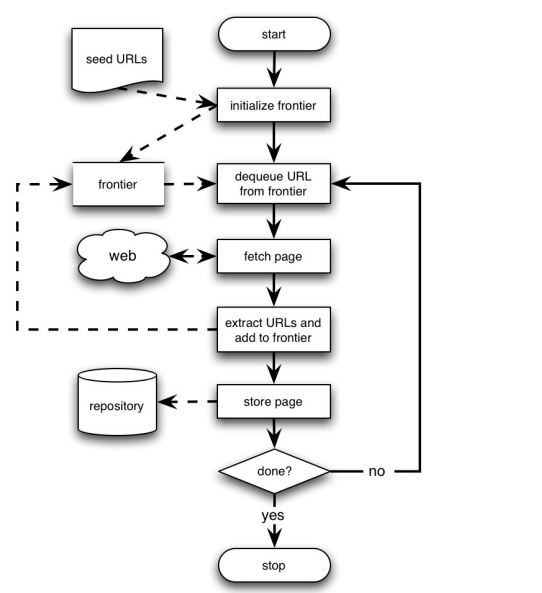
\includegraphics[scale=1.0]{CrawlerAlgorithFlowchart}
		\caption{Crawler Breadth search Flowchart}
		\label{fig:CrawlerAlgorithFlowchart}
	\end{figure}
	Crawler used here is sequential cralwer. If we closely look at flowchart the order of page visits is closely related to frontier data structure and is determined with it. There can be list of starting URLs which here in flow chart is Seeds.
	
	Once the download is completed, collection of stored repository stores web page. Link extractor gets the page, which then parse the page HTML content which extracts hyper-links contained within. Related URLs are passed to URL distributor, which assigns each URL to a crawling process. Most of the hyper links refer to pages on same website, assignment to local crawling process is common case. Now the URL is passed through URL filter and into the duplicate URL eliminator, which in turn maintains set of all URLs.  At last URL priotizer selects a position for the URL in the frontier, based on factors such as estimated page importance or rate of change.
	
	Web Crawler needs to keep track of URL which are already visited and which needs to be visited. Each URL is associated with a flag whether page is downloaded or not. There are few of the key functions which should be taken into consideration such as Retrieving a URL, marking a URL as downloaded, adding a new URL and testing whether the set contains a URL. Modern web Crawler are splits into two main data structures as. 
	\begin{enumerate}
		\item To maintain the set of URL that have been visited (duplicated URL eliminator)
		\item To maintain set of URL that has to be visited (frontier)
	\end{enumerate}
	
	\subsubsection{Frontier Data Structure}
	First in First out (FIFO) is implemented with  Frontier Data structure. Breadth-first traversal of web graph is used as search technique. FIFO queue has long runs of URLs on same web server because most of the  hyper-links are relative. Multiple overlapping request to server are not issued as they are not so common. It can be easily realized with maintaining a mapping between web servers and crawling threads. A separate FIFO queue is assigned to each crawling thread. One more dedicated policy which can be used is, to send request to each web server depending on server's capabilities. For example crawler can delay requests to a server by a multiple of time to get the last page from server. Mercator web crawler implements adaptive politeness. Frontier is divided into two parts, "front end" and "back end".
	
	Single queue Q and URLs are added to the frontier by enqueuing them into that queue. Separate queues are contained in back end. Queue containing URL belongs to a single web server; mapping from back-end queues to web servers are maintained on table T. In addition, associated with each back-end queue q was a time t at which the next URL from q may be processed. These (q,t) pairs were organized into an in-memory priority queue, with the pair with lowest t having the highest priority.  Removing highest-priority entry (q,t) obtained URL by crawling thread from priority queue, waiting if necessary until time t had been reached, dequeuing the next URL u from q, downloading it, and finally reinserting the pair (q,tnow + k * x) into the priority queue, where now is the current time, x is the amount of time it took to download u, and k is a "politeness parameter"; typically 10. If dequeuing u from q left q empty, the crawling thread would remove the mapping from host(u) to q from T, repeatedly dequeue a URL u from Q and enqueue u into the back-end queue identified by T(host(u)), until it found a u such that host(u) was not contained in T. At this point, it would enqueue u in q and update T to map host(u) to q.
	
	Web crawlers may also want to prioritize the URLs in  frontier as adding politeness policies that govern the rate at which pages are downloaded from web site. Crawling pages is desired according to estimated usefulness. A crawler can structure the frontier as a disk based priority queue ordered by usefulness. A URL is assigned as discrete priority level and inserted into the corresponding queue. To dequeue a URL either the highest priority non-empty queue is chosen, or a randomized policy biased toward higher-priority queue is employed.
	
	\subsubsection{URL Seen Test (duplicated URL eliminator)}
	URL Seen Test is used to remove adding various instances of the similar URL to the frontier and therefore it is called duplicate URL eliminator. Insertion and set membership testing is supported by UST during batch crawling setting. Bloom filter and hash table are few of the implementation of UST. In memory implementation has issues with scaling to large web corpora but they scale well in frontier. Distributed crawlers and a hash table realizing the UST are employed by commercial search engines which can be partitioned across the machines in the crawling cluster.
	
	UST state must reside on disk if memory is at a premium. Disk seek is required by each lookup search, severely limiting the throughput. Throughput can be increased by about an order of magnitude\cite{Graphstructure} to few thousand lookups per second by caching popular URLs. Even though the latency of disk seeks is poor, the bandwidth of disk reads and writes are high. Performing random file access is fairly poor but streaming sequential reads can be reasonably good. Single batch with Mercator crawler are inserted with various lookup and insertion operations. Mercator does processing of each batch by sequentially reading a set of sorted URL hashes from disk and writing them out to a new File\cite{Highperformancewebcrawling}
	
	Reading the old hash file and writing out an updated version involves adding a bunch of URL into disk-based hash files. Hence, the required time is directly equivalent to the number of discovered URLs. To store the URL hashes on disk in sorted order as before can be considered as slight improvement of this pattern, but lightly packed rather than densely packed. The k highest-order bits of a hash determine the disk block where this hash resides. Merging a batch into the disk file is done in place, by reading a block for which there are hashes in the batch, checking which hashes are not present in that block, and writing the updated block back to disk. Thus, the time requirement for merging a batch is proportional to the size of the batch, not the number of discovered URLs. Once any block in the file fills up completely, the disk file is rewritten to be twice as large, and each block contains hashes that now share their k + 1 highest-order bits.
	
	\subsubsection{Auxiliary Data Structures}
	A Robots Exclusion protocol should be followed by web crawlers, it is a protocol which makes a web site admins to bar crawlers from crawling. It is accomplished by providing a file at URL/robots.txt containing rules such as which pages the crawler is allowed to download. Before crawling an web site, Crawler must check if the web site supplies /robots.txt file and if it does, crawler should adhere to rules. Using some cache eviction policies entries must be discarded. Additionally web servers can specify an expiration time for their /robots.txt file. Some URLs contain a host component (e.g., www.yahoo.com), which is "resolved" using the Domain Name Service (DNS). Due to request forwarding nature of protocol, DNS requests can take quite a long time. Therefore, crawlers often maintain their own DNS caches. As with the robots exclusion rule cache, entries are expired according to both a standard eviction policy, and to expiration directives. The robots.txt file must be fetched from a website so that URL under consideration passes the robot restrictions and hence can be added to URL frontier. By performing the filtering during the link extraction process, we would have especially high locality in the stream of hosts that we need to test for robots.txt files, leading to high cache hit rates. A URL may be in frontier for days or even weeks.
	
	\subsubsection{Distributed crawling}
	
	Web crawler can be distributed over multiple machines which will help in increasing the throughput of crawling. By partitioning the URL space, Distributed crawling can be achieved  i.e. node is responsible for a subset of the URLs on the web. URL space is best partitioned across web site boundaries. Using partitioning the URL across site boundaries, Politeness policies can be best achieved . In addition, most of the major data structures can be easily partitioned across site boundaries, i.e. the frontier, the DUE, the DNS and robots exclusion caches of each node contain URL, robots exclusion rules, and name-to-address mappings associated with the sites assigned to that node, and nothing else.
	
	Using crawling process web pages are extracted and downloaded  with the help of prevalence relative links on web, links will be responsible for large majority of extracted URLs. Forwarding of URLs can be done through peer to peer TCP connections\cite{Highperformancewebcrawling}, a shared file system\cite{Highperformance}, or a central coordination process\cite{anatomy}. By maintaining a cache of popular URLs, used to avoid repeat forwarding\cite{Graphstructure}, the amount of communication with other crawler nodes can be reduced . A variant of distributed web crawling is peer to peer crawling which spreads crawling over a loosely collaborating set of crawler nodes. There are two types of policies used under distributed crawling:
	\begin{enumerate}
		\item Dynamics assignment: A central server assigns new URLs to different crawlers dynamically under dynamics assignment policy. To dynamically balance the load of each crawler, Central servers are used. Typically the systems can add or remove downloaded processes. Most of the workload must be transferred to the distributed crawling process for large crawls.
		\item Static assignment: Within this policy, there is a fixed rule stated from the beginning of the crawl that defines how to assign new URLs to the crawler. To transform URLs into a number that corresponds to the index of the corresponding crawling process, hashing function can be used.
	\end{enumerate}
	\subsubsection{Incremental crawling}
	Snapshots of batch crawling can be combined using Web crawlers. To perform incremental or continuous crawling where the resources of the crawler are divided between downloading newly discovered pages. Few changes to the major data structures of crawlers are required for making good incremental crawling. DUE should support deletion of URLs that are no longer valid. If URL are prioritized in frontier, the priority of a previously downloaded URL should be dependent on a model of the page's temporal behaviour based on past observations. Other factors such as page quality are also taken into account. By augmenting URLs in the frontier with additional information in particular previous priorities and compact sketches of their previous content, the functionality is best facilitated. This extra information allows the crawler sketches of their previous content. Three possible metrics that are most popular are as below:
	\begin{enumerate}
		\item Coverage: count the number of pages that exist on the web but are not present in the repository at any given time.
		\item Freshness: count the number of documents that are present in the repository, but whose content was
		changed after insertion into the repository. Alternatively, the metric may incorporate a measure of the
		size of the change for individual pages.
		\item Age: the average age of documents in the repository (e.g., time since they were last updated).
	\end{enumerate}
	To reflect their relative importance for the application, above metrics can be adjusted to add weights of autonomous pages. Documents which are dominated by thousands of other documents for every possible query should probably be weighted lower than documents that are often found by users of the search engine. The quality of an incremental crawling strategy must also be evaluated on the basis of resources that it consumes in order to maintain a given level of metric.
	\subsection{Browser automation: Selenium}
	There are numerous browser automation tools available such as Kantu, QF-Test, Sahi, SOAtest, iMacros, Selenium and so on. Kantu can automate website by taking screenshots. It helps to visually automate tasks and makes web automation intresting. Using Kantu soutions can be created for web automation, web scraping or web testing in just few minutes. It works on the visual website similar to how we human does. Kantu's visual approach speeds up web automation projects tenfold. But
	Kantu uses only screen shots as scripting language and not CSS or DOM object which is needed in our project work. QF-Test is a cross platform software tool for the GUI test automation and specializes in automating test cases rather than any implementation of a Task. QF-Test's capture/replay function enables recording of tests for beginners, while modularization allows for creating large test suites in a concise arrangement.  QF-Test uses visual scripting, Jython and Groovy as scripting language. Sahi uses it's own Sahi script whereas Selenium supports Ruby, Java, NodeJS, PHP, Perl, Python, C\#, Groovy as scripting language. 
	
	In addition, the web driver provided by Selenium for Internet Explorer is very reliable, sophisticated and most important it is Open source. Because of added advantage, selenium was chosen to work on.
	Selenium\cite{AutomationTestingAnIntroductiontoSelenium} is a browser automation tool; mostly used to simulate user interaction on web applications. The browser control is automated so that repetitive tasks can be easily achieved with it. One of Selenium's key features is the support for executing one's tests on multiple browser platforms. Selenium,  is a combination of selenium IDE, selenium Web driver and selenium gird. Selenium grid helps to use the selenium APIs to control browser instances distributed over a grid of machines. Selenium IDE is an extension for Firefox used to record and playback tests. Selenium uses lot of Jargon.
	
	\begin{enumerate}
		\item Selenium core JavaScript that control the browser.
		\item Selenium WebDriver binds both language binding and individual browser controlling core.
		\item Selenium RC is used for language binding.
	\end{enumerate}
	
	Variant of selenium:
	\begin{enumerate}
		\item Selenium IDE
		\item Selenium Core
		\item Selenium Remote Control
		\item Selenium Grid
	\end{enumerate}
	
	Selenium\footnote{http://www.seleniumhq.org/docs/01\_introducing\_selenium.jsp\#test-automation-for-web-applications} consist of different software tools each with a different approach to supporting browser automation. The entire set of tools results in a rich set of testing functions specifically geared to the needs of automation of web application of all types. Such operations are highly flexible allowing many options for locating UI elements and comparing expected test results against actual application behaviour. While selenium is a tremendous tool it isn't without drawbacks.
	There are also few downfalls of Selenium which is important to maintain here.
	\begin{enumerate}
		\item	There can be cases when selenium fails to recognize objects
		\item Online support for selenium is very less
		\item Because of its Java-script based automation engine and the security limitations browsers apply to Java-script, different things became impossible to do.
	\end{enumerate}
	But later years Selenium introduced Webdiver which talks directly to web browser and avoids Java-script dependency. Good thing about selenium is it's wide popularity and large community support. Few of the advantages of Selenium are:
	\begin{enumerate}
		\item Opensource tool
		\item No licensing cost
		\item Customize according to our requirement
	\end{enumerate}
	WebDriver were the tool of the future. The joining of the two tools provided a common set of features for all users. Webdriver addresses some shortcoming in selenium partly because selenium contributors and felt that it was the best way to offer users the best possible framework.
	\subsubsection{WebDriver Design}
	WebDrivers API \cite{SeleniumTestingFramework} is also called as  object-based. The interfaces are very well defined and try to manage single responsibility and therefore rather than modelling every single possible HTML Tag, We have only one WebElement interface. Snippet of code for initialization of web driver\footnote{http://www.aosabook.org/en/selenium.html} is shown below.
	\begin{lstlisting}
	WebDriver driver = new FirefoxDriver();
	driver.<user hits space>
	driver.findElement(<user hits space>);
	driver.findElement(By.id("someid"));
	\end{lstlisting}
	Most of the IDEs will now drop a hint about the type of the argument expected. There are a number of preconfigured factory methods for "By" objects as static methods on the by itself. For example, there is a JavascriptExecutor interface that is built with the ability to execute arbitrary chunks of Java-script in the context of the current page. A successful cast of a WebDriver instance to that interface indicates that you can expect the methods on it to work.
	\subsubsection{The IE Driver}
	Number of COM interfaces working in concert helps to build IE browser. JavaScript window is an IHTMLWindow.document is an instance of the COM interface IHTMLDocument. Good thing about IE is that if COM classes works with IE6 it will still continue to work with IE9.
	
	IE's main positives is, it does not need to have installer. So if there are no installer, there are consequences to this choice. IDE drivers built for selenium are tightly integrated with C\#. It is not an good option to do the bulk of the coding in C\#, Even though it is an attractive language . Something native for the communication to IE should be considered and therefore C++ and the main reason for choosing it could be because of no need to use primary Interloop Assemblies (PIAs). Since we would need to run an installer in order to make that DLL available, we would link our library for communication with IE. In the figure  \ref{fig:OriginalIEdriver}, design of IEDriver is shown 
	\begin{figure}[h]
		\centering
		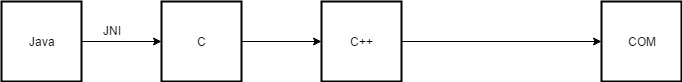
\includegraphics[scale=0.6]{OriginalIEdriver}
		\caption{Original IE driver}
		\label{fig:OriginalIEdriver}
	\end{figure}
	Looking at the diagram IE COM, automation interfaces are being used and hence to make it easier to manage raw interfaces are wrapped with set of C++ classes that closely mirrored WebDriver API. JNI is being used for Java classes to communicate with C++. This approach works well with java being only client language but could be very difficult if every other language would require to change the underlying library and therefore it is considered not the correct way for abstraction. Every other language had a mechanism of calling down straight C code. In c\# it is PInvoke, In ruby it is FFI, python has ctypes and Java it is JNA (Java Native Architecture). API has to be exposed to lowest common denominator and it was done by taking object model and flattening it, using a simple two or three letter prefix to indicate the "home interface" of the method: "wd" for "WebDriver" and "wde" for WebDriver Element. In Figure 
	\ref{fig:ModifiedIEdriver}, design is shown 
	\begin{figure}[h]
		\centering
		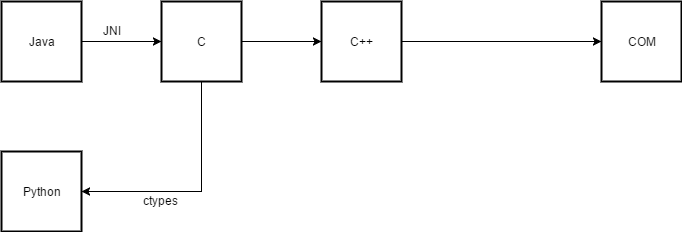
\includegraphics[scale=0.6]{ModifiedIEdriver.PNG}
		\caption{Modified IE driver}
		\label{fig:ModifiedIEdriver}
	\end{figure}
	On the Java side, this library of functions is exposed via an interface, which we then adapted to make it look like the normal object-oriented interface presented by WebDriver. For example, the Java definition of the getAttribute method looks like:
	
	\begin{lstlisting}
	public String getAttribute(String name) {
	PointerByReference wrapper = new PointerByReference();
	int result = lib.wdeGetAttribute(
	parent.getDriverPointer(), element, new WString(name), wrapper);
	errors.verifyErrorCode(result, "get attribute of");
	return wrapper.getValue() == null ? null : new StringWrapper(lib, wrapper).toString();
	}
	\end{lstlisting}
	
	More and More of IE driver is being moved to sit upon the same automation Firefox. To achieve this we compile each of the atoms as c++ header file, exposing each function as constant. At last, we only have Interaction of API's in native code and rely on the atoms as much as possible.
	\subsubsection{The Remote Driver}
	Remote driver mechanism is used to reduce the cost of maintaining web Driver by providing a uniform interface that language binding can code against. To communicate with browser instance that is running out of process Remote driver is used. RPC mechanism is divided into two: transport and encoding. First iteration of the design was developed as a part of Firefox driver.
	
	Mozilla, and therefore Firefox, is always seen as being a multi-platform application by its developers. Mozilla created a framework that allowed components to be built and bolted together called XPCOM (cross-platform COM) is inspired by Microsoft's COM.  IDL declares XPCOM interface, language binding for C and other languages and JavaScript as well as other languages are available. It's possible to make use of XPCOM objects in Firefox extensions because of the XPCOM consisting of JavaScript.
	
	Custom protocol does not have any of the libraries available, hence they have to be built from the ground up for every language that we wanted to support. When we used to send only text line oriented protocol it was fine but when sending images started it was tedious.
	
	Original RPC mechanism wasn't that practical and hence alternative mechanism for this was widely spread called HTTP. The Firefox driver is implemented as a Firefox extension, the basic design of which is shown in Figure \ref{fig:Flowchart}\footnote{https://github.com/SeleniumHQ/selenium/wiki/FirefoxDriver}. HTTP server has been embedded into it. Writing HTTP servers in XPCOM wasn't one of core areas to work on, so when the available resources joined it was replaced with a basic HTTPD written by Mozilla themselves. Requests are received by the HTTPD and almost straight away passed to a dispatcher object.
	\begin{figure}[h]
		\centering
		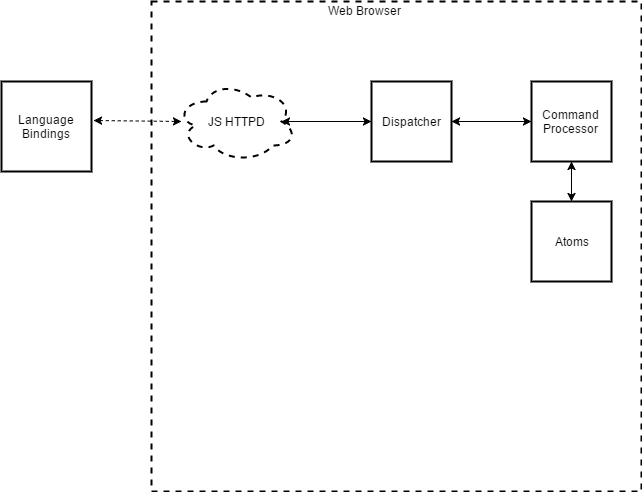
\includegraphics[scale=0.6]{SeleniumHttp.PNG}
		\caption{Firefox Driver Architecture}
		\label{fig:Flowchart}
	\end{figure}
	For example Json Object shown below is then passed as a JSON string to a custom XPCOM component written called the CommandProcessor. Code snippet below is for reference:
	\begin{lstlisting}
	{
	'name': 'getElementAttribute',
	'sessionId': { 'value': 'XXX' },
	'parameters': {
	'id': 'some_opaque_key',
	'name': 'rows'
	}
	}
	var jsonResponseString = JSON.stringify(json);
	var callback = function(jsonResponseString) {
	var jsonResponse = JSON.parse(jsonResponseString);
	if (jsonResponse.status != ErrorCode.SUCCESS) {
	response.setStatus(Response.INTERNAL_ERROR);
	}
	response.setContentType('application/json');
	response.setBody(jsonResponseString);
	response.commit();
	};
	// Dispatch the command.
	Components.classes['@googlecode.com/webdriver/command-processor;1'].
	getService(Components.interfaces.nsICommandProcessor).
	execute(jsonString, callback);
	}
	\end{lstlisting}
	Object above in code is converted into JSON string. A callback to the execute method that causes the HTTP response to be sent is passed.
	
	The determination of which function to call is being done with the help of "name" which is been looked by execute method of the command processor. The first parameter given to this implementing function is a "respond" object, which encapsulates not only the possible values that might be sent, but also has a method that allows the response to be dispatched back to the user and mechanisms to find out information about the DOM. The second parameter is the value of the parameters object seen above (in this case, id and name). The advantage of this scheme is that each function has a uniform interface that mirrors the structure used on the client side. This means that the mental models used for thinking about the code on each side are similar. Here's the underlying implementation of getAttribute,
	
	\begin{lstlisting}
	FirefoxDriver.prototype.getElementAttribute = function(respond, parameters) {
	var element = Utils.getElementAt(parameters.id,
	respond.session.getDocument());
	var attributeName = parameters.name;
	
	respond.value = webdriver.element.getAttribute(element, attributeName);
	respond.send();
	};
	\end{lstlisting}
	
	In order to make element references consistent, the first line simply looks up the element referred to by the opaque ID in a cache. Opaque ID is a UUID and the "cache" is simply a map with respect to Firefox driver. Referred to element is both known and attached to the DOM is checked with the help of getElementAt method. If either check fails, the ID is removed from the cache (if necessary) and an exception is thrown and returned to the user.
	The second line from the end makes use of the browser automation atoms discussed earlier, this time compiled as a monolithic script and loaded as part of the extension.
	In last line, the send method is called. Simple check is done that only send a respone once before it calls the callback given to execute method. The response is sent back to the user in the form of a JSON string, which is decanted into an object that looks:
	\begin{lstlisting}
	{
	'value': '7',
	'status': 0,
	'sessionId': 'XXX'
	}
	\end{lstlisting}
	Browsing the web in a copy of Firefox with the WebDriver extension installed will result in a bad security feature as it makes it trivially easy for someone to remotely control the browser.
	There is a DOM messenger, waiting for the webdriver Command that reads the serialized JSON object and calls the execute method on the command processor. The callback is one that simply sets the response attribute on the document element and then fires the expected webdriverResponse event.
	
	\subsubsection{Combinatorial Explosion}
	To minimize cost of maintenance with X browsers supporting Y languages is always an challenge, it would be trap of maintaining X*Y implementations. There can be a way to reduce the number of language that web driver support. It's always better to write automation scripts in the same language that they work on. There is also a way of reducing the supported browser but it will also not be a feasible solution.
	
	It is not a feasible solution to reduce the number of languages that webdriver supports which would be one way to reduce the cost. It is always advantageous to use the framework to be able to write test in same language as the development in. One of the better measure to tackle with language binding is to try and make all the browsers look identical to the language bindings: a uniform interface should be offers so that it can be addressed easily in a wide variety of languages. IE driver has successfully pushed the responsibility for locating and starting IE into the main driver logic. Java world alone, this means that three major classes that handle configuring and starting Firefox weighing in at around 1300 lines of code. Although this has resulted in a surprising number of lines of code being in the driver, the language binding for creating a new instance boils down to a single method call into that driver. For comparison, the Firefox driver has failed to make this change. These classes are duplicated in every language binding that wants to support the FirefoxDriver without relying on starting a Java server. That's a lot of additional code to maintain.
	
	\subsubsection{Layers and Javascript}
	Broswer automation tool is built of three parts:
	\begin{enumerate}
		\item Some way of emulating user input
		\item Mechanism for executing Javascript
		\item A way of interrogating the DOM
	\end{enumerate}
	We try to analyse the way or mechanism which can be used to interrogate the DOM. The language of browser is JavaScript, which is a perfect language to use when testing the DOM. But when working with JavaScript posses some interesting challenges and competing requirements which needs balancing.
	
	Layered set of libraries are used in selenium. Google's closure library is the bottom layer, which supplies primitives and mechanism allowing sources files to be kept focused and as small as possible. Simple tasks such as getting the value of an attribute through determining whether an element would be visible to an end user such as simulating a click using synthesized events are undertaken using utility library. Within the project, these are viewed as offering the smallest units of browser automation, and so are called browser automation toms or atoms. 
	Figure\ref{fig:LayersofSeleniumJSLibrary}\footnote{http://www.aosabook.org/en/selenium.html} shows layers of selenium JavaScript library.
	
	There are adapter layers that compose atoms in order to meet the API contracts of both Webdriver and Core. The modularization techniques used by libraries are understood bc closure compiler. The output language as Java is targeted by Closure Compiler. It is so simple to order input files so that it can be considered as "Compilation", advanced minification and dead code removal. People working with Closure Library are very much familiar with JavaScript as language. atomic library of code is used pervasively throughout the project if there is an requirement to interrogate the DOM. There is an monolithic script used for RC and those divers largely composed of JS. It allows the JavaScript to be pushed into the underlying driver without needing to expose the raw source in multiple places. It's possible to manage consistent behaviour between different browsers and at the same time library written in Java is easy and fast as the atoms are used extensively. Closure library can load dependencies dynamically and hence there is only need for selenium developer to write and a test and load it in browser. Abstraction is done very well with Closure library, there are continuous builds to run test in supported browser.
	\begin{figure}[h]
		\centering
		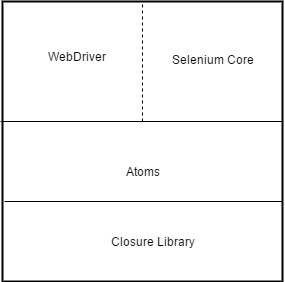
\includegraphics[scale=0.6]{LayersofSeleniumJSLibrary}
		\caption{Layers of Selenium Javascript Library}
		\label{fig:LayersofSeleniumJSLibrary}
	\end{figure}
	Several architectural themes of the project are viewed by atoms. Implementation of an API to be easy going with JavaScript should be available. The bus factor of project is used by atoms which makes it more favourable. JavaScript unit test case can be used which act as a barrier to joining the Open Source project can be used to check if a fix works , hence the task of writing layer is both easier and more accurate.
	\subsubsection{Different Browsers}
	Web browser is a translation device, which takes document written in HTML language and translates it into a formatted web page. The basic rules for translating HTML documents are established by the WWW. HTML standards usually run ahead of that the browsers support. Over the past few years Internet Explorer has done a lot than Opera or other browsers. An overview of all the supported browser with Selenium automation tool are shown in Table \ref{SB}.
	\begin{table}[H]
		\centering
		\begin{tabular}{|l|l|l|l|}
			\hline
			\textbf{Browser} & \textbf{Selenium IDE} & \textbf{Selenium 1 (RC)} 
			& \textbf{Operating Systems}\\ \hline
			Firefox 3.x   & Record and playback tests             & Start browser, run tests  & Windows, Linux, Mac    \\ \hline
			
			Firefox 3  & Record and playback tests             & Start browser, run tests  & Windows, Linux, Mac    \\ \hline
			
			Firefox 2  & Record and playback tests             & Start browser, run tests  & Windows, Linux, Mac    \\ \hline
			
			IE 8  & Test execution only via Selenium RC             & Start browser, run tests  & Windows    \\ \hline
			
			IE 7  & Test execution only via Selenium RC             & Start browser, run tests  & Windows    \\ \hline
			
			IE 6  & Test execution only via Selenium RC             & Start browser, run tests  & Windows    \\ \hline
			
			Safari 4  & Test execution only via Selenium RC             & Start browser, run tests  & Windows, Mac    \\ \hline
			
			Safari 3  & Test execution only via Selenium RC             & Start browser, run tests  & Windows, Mac    \\ \hline
			
			Safari 2  & Test execution only via Selenium RC             & Start browser, run tests  & Windows, Mac    \\ \hline
			
			Opera 10  & Test execution only via Selenium RC             & Start browser, run tests  & Windows, Linux, Mac    \\ \hline
			
			Opera 9  & Test execution only via Selenium RC             & Start browser, run tests  & Windows, Linux, Mac    \\ \hline
			
			Opera 8  & Test execution only via Selenium RC             & Start browser, run tests  & Windows, Linux, Mac    \\ \hline
			
			Google Chrome  & Test execution only via Selenium RC             & Start browser, run tests  & Windows, Linux, Mac    \\ \hline
			
			Others  & Test execution only via Selenium RC             & Partial support possible  & As applicable    \\ \hline
		\end{tabular}
		\caption{Overview of Supported browsers by Selenium}
		\label{SB}
	\end{table}
	HTML tags isn't universal, you could be building your pages with parts of the language that not all browsers understand. In such cases browser will ignore that part of your page it can translate and way pages will be displayed is affected.
	
	\subsubsection{Extensibility and Flexibility}
	Selenium is highly flexible. Functionality could be added to selenium test scripts and selenium's framework to customize test automation. This particular use case is the greatest strength when compared with other automation tools. One more good point is as selenium is open source, the sourceode can always be downloaded and modified.
	\subsection{OpenDiabetesVault Architecture and Data slicing}
	\label{subsec:OpenDiabetesVaultArchitecture}
	To help understand the motivation for performing Data slicing, it is very important to understand the project OpenDiabetesVault-engine. This is well illustrated with the help of Architecture Diagram as shown in figure \ref{fig:ODVArchitecture} which is very much self explanatory. The overall view of Architecture shows that OpenDiabetesVault (ODV) consist of four main modules as Geathrering, Import, Interpreter and Export which can be furtherer divided into sub modules. Revisiting the main goal of ODV is to perform Data analysis on extracted data from different sources. If we take a look at Geathering module, it is subdivided into Medtronics crawler, Google Time-line, Smart band and Glucosio plug-in. For instance Medtronics module has responsibility of extracting data from carelink website and present it in CSV format which is main part of this thesis. Once the data is extracted it gets into import module where all the CSV data is combined with the help of interpreter which act as an type of data coming from which source and how it is related. At the end of module 2 and 3 i.e Import and Interpreter we have a huge dataset containing data bundled from all the available sources and ready for analysis.
	\begin{figure}[h]
		\centering
		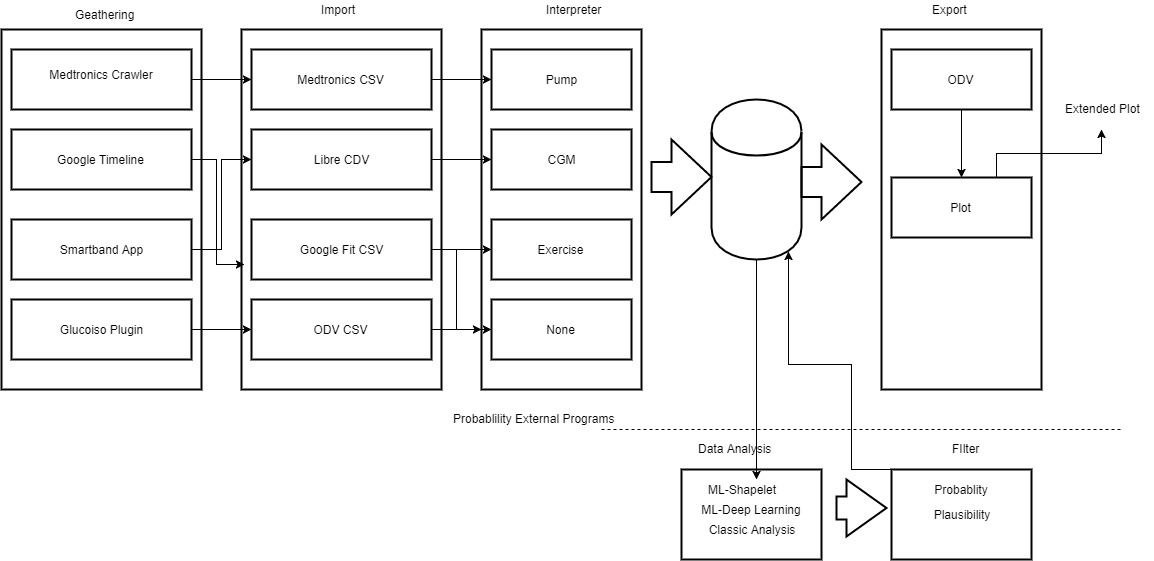
\includegraphics[scale=0.4]{ODVArchitecture.jpg}
		\caption{ODV Architecture}
		\label{fig:ODVArchitecture}
	\end{figure}
	
	Data analysis is the process by which data is evaluated with the help of analytical and logical reasoning of the provided data. Data from various sources is gathered, reviewed and analysed to generate pattern or conclusion. But to generate some conclusion data should be of very high quality. However very rarely data generated from different sources has such quality and hence pre work for "cleaning"/"cluttering" of irrelevant data has to be taken place. For instance "cleaning" is the process of removing invalid data from datasets which are either
	\begin{enumerate}
		\item Incorrect values for specific variables.
		\item Cases in the data who met exclusion criteria and should not be in the study.
		\item Duplicate cases
		\item Skip-pattern or logic breakdowns
	\end{enumerate}
	Quality of data mainly involves human judgement to decide which points are valid and which are not, and hence there is a huge chance of valid data points caused by some effect not sufficiently accounted for in the hypothesis/assumption behind the analytical method applied. Data quality measures the amount of consistency, instance correctness, completeness and minimality achieved in a certain system. Table \ref{DataQuality} \cite{Dataquality} shows data quality added from the view of data mining.
	
	\begin{table}[H]
		\centering
		\begin{tabular}{|p{3cm}|p{5cm}|p{7cm}|}
			\hline
			\textbf{Requirement} & \textbf{Explanation} & \textbf{Dirty Data Examples} 
			\\ \hline
			Correctness   & Data reflect its true reality             & Age=120 or input birthday= "11/11/1911" when birthday is unknown\\ \hline
			
			Completeness   & Data sets contain all data mining needs & Lack lost customers information while mining customer retaining\\ \hline
			
			Consistency  & Codes in different systems are consistent; no conflict while
			integrating  & A customer’s ID in CRM system is "1100", while in POS system is "021233"\\ \hline
			
			Minimality  & No repeat records after integration  &A sales record became 3 records after integration\\ \hline
			
			Reliability  & Results of integrating stable regardless of who or when did  & Attributes in product table changed between two integrating process resulting in confused sales information\\ \hline		
		\end{tabular}
		\caption{Data quality added from the view of data mining}
		\label{DataQuality}
	\end{table}
	
	A lot of time is spent on data cleaning and preparing data, up to 80 percent \cite{TinyData} of the time is usually spent in a project and ODV architecture is no different. Much of the importance within the ODV architecture is given in cleaning the data so that researchers in TK lab implementing Data analysis techniques will deal with high quality of data. The objective is to structure the data to facilitate the data analysis you set out to perform. In such situation we have found out that Data entries i.e rows from dataset needs to be sliced in such a way so that onyl relevant data is moved to next level for analysis. To get this focused data we used DataSlicer. As shown in the figure \ref{fig:ODVArchitecture} it takes data from the data base, some options and some filters produces a list with time points where events occur specified by the filter. The goal of filters is to achieve data quality with most of the below mentioned criteria
	\begin{enumerate}
		\item Accuracy
		\item Completeness
		\item Accessibility
		\item Reliability
		\item Relevance.
		\item Consistency across data sources
		\item Update status
	\end{enumerate}
	As shown in the figure \ref{fig:Dataslicer}\footnote{https://github.com/OpenDiabetes/OpenDiabetesVault-engine/wiki/Data-Slicing} it takes data from the data base, some options and some filters which is a type of complex Event process \cite{EventProcessing} and produces a list with time points where events occur specified by the filter. Filters can be registered at the DataSlicer and implement the Filter interface. The filters are combined with the logical and paradigm. As shown in the figure below, filters take a data array together with options. The filter will delete not matching data from the array and returns it together with a list of time spans where continuous data is present (this could be used to find the data in the complete array again). 
	\begin{figure}[h]
		\centering
		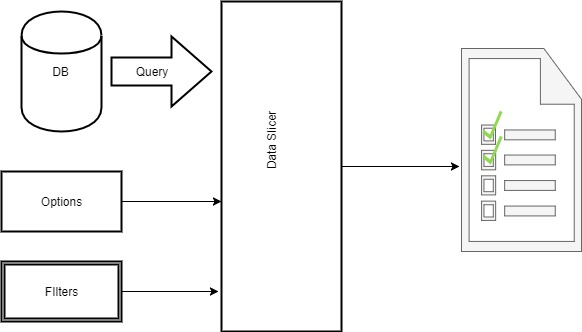
\includegraphics[scale=0.7]{Dataslicer.jpg}
		\caption{Data Slicer}
		\label{fig:Dataslicer}
	\end{figure}
	
	Most of the work for Data slicer is done with the help of Filters. Data Filtering\footnote{https://github.com/OpenDiabetes/OpenDiabetesVault-engine/wiki/Data-Filtering} are the one which implement different data cleaning and data cluttering methodologies. For data filtering we provide the Filter interface. Filters can be registered at processing services like the DataSlicer and have to implement the Filter interface. Multiple filters are combined with the logical "and" paradigm. As shown in the figure \ref{fig:Filters}, filters take a data array together with options. The filter will delete not matching data from the array and returns it together with a list of time spans where continuous data is present (this could be used to find the data in the complete array again).  An overview of Data Filtering is shown in figure \ref{fig:Filters}.
	\begin{figure}[h]
		\centering
		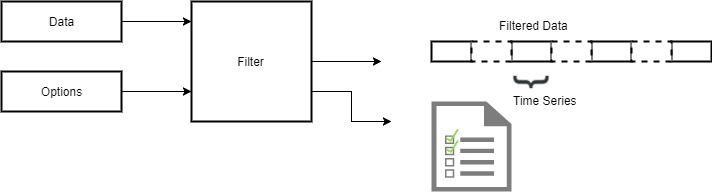
\includegraphics[scale=0.7]{Filters.jpg}
		\caption{Data Filtering}
		\label{fig:Filters}
	\end{figure}
	Filters in our Thesis work can be broadly classified as Time related Filters and
	Threshold related Filters. Time-Related Filters as shown in figure \ref{fig:TimeRelated} consist of Timespan Filter and TimePoint Filter. This kind of filters are used to generate a time point or a time span where some kind of event happens or some kind of data is available or not. For instance, if you want to check the basal insulin rate you search for time spans where no bolus is given. Filters of the time point type should provide a margin option enable data observation around the found point. They are used to retrieve data within a given time span or time point.
	\begin{figure}[h]
		\centering
		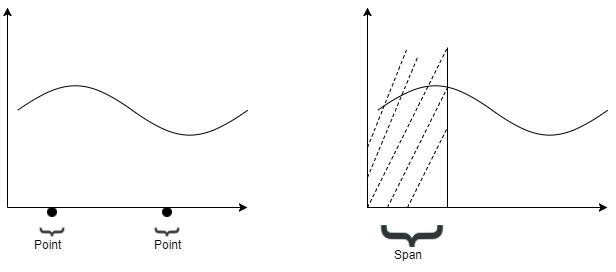
\includegraphics[scale=0.7]{TimeRelated.jpg}
		\caption{Time Related Filtering}
		\label{fig:TimeRelated}
	\end{figure}
	Moving from Time-Related Filter, there is another type of filer called Threshold-Related Filter as shown in figure \ref{fig:Threshold}. Threshold related filters are used for filtering data within a given Filter type and if that data point is under or threshold value given as input from user. The steps followed to achieve Over or Under Threshold is something like below.
	\begin{figure}[h]
		\centering
		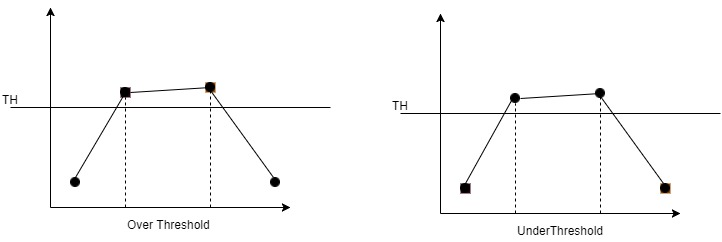
\includegraphics[scale=0.7]{Threshold.jpg}
		\caption{Threshold Filtering}
		\label{fig:Threshold}
	\end{figure}
	\begin{enumerate}
		\item First check if given data i.e a row from a data set, having column as Type matched with Filter Type mentioned in options(argument from user).
		\item If the entry set i.e a row matched with a filter type, then this row is sent to check if that row has value under or above Threshold value.
		\item If it does then entry is added to list with return type as FilterResult.
		\item FilterResult consist of EntryValue Type and Pair of Date,Date.
	\end{enumerate}
	Filters also consist of an GenericAvailableFilter class which takes VaultEntryType and FilterType as argument. This class is helper class for Threshold filter class to return dataset which matched with FilterType value. If particular entry in dataset matches with the type mentioned in argument, That entry will be added to list which will further passed to filter.
	\subsection{Unit Testing}
	Unit Testing\cite{EffectivnessofUnitTest} is testing modules of code in isolation with test code. It is a way to test the behaviour and functionality of your system. The main goal of our unit testing is to take the smallest piece of software module in the application, isolate it from the remainder of code and determine whether it behaves exactly as you expect. Each unit is tested separately before integrating them into modules to test the interfaces between modules. Unit testing has proven its value in that a large percentage of defects are identified during its use. The benefit of unit test cases are:
	\begin{enumerate}
		\item Properly unit tested code can be cleaned up with little chance of breaking anything without noticing it.
		\item It gives confidence to developers when adding or making changes to code.
		\item It helps to document the code.
		\item It indicates methods and classes that are integrated 
		\item Indicated code that are tightly coupled
		\item Provide a means to use your API and look for difficulties early on 
	\end{enumerate}
	Performing unit testing is designed to be simple, generally the tests are written in the form of functions that will determine whether a returned value equals the value you were expecting when you wrote the function (or the value you will expect when you eventually write it - this is called Test Driven Development when you write the tests first). Figure \ref{fig:Testingmethodologies} shows different Testing methodologies and the hierarchy of their usage
	\begin{figure}[h]
		\centering
		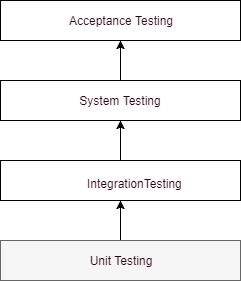
\includegraphics[scale=0.7]{Testing.jpg}
		\caption{Testing Methodologies}
		\label{fig:Testingmethodologies}
	\end{figure}
	By doing unit testing we also force the design of the software into something that is unit testable. Many people are of the opinion that this design is for the most part Good Design regardless of other benefits from testing. So one reason to do unit test is to force your design into something that hopefully will be easier to maintain than what it would be had you not designed it for unit testing. It is that level of software testing where units/ components of a software are tested. Most of the time unit testing is performed using the White Box Testing. Software developers themselves or their peers perform Unit Testing. Sometimes it can also be performed by independent software testers. Figure \ref{fig:UnitTesting} shows Unit Testing and the process of acheiving it.
	\begin{figure}[h]
		\centering
		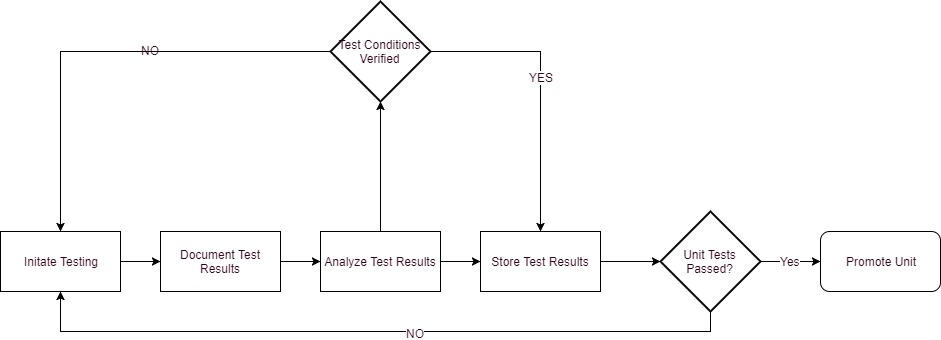
\includegraphics[scale=0.5]{UnitTesting.jpg}
		\caption{Unit Testing}
		\label{fig:UnitTesting}
	\end{figure}
	
	The side effect can be that developers test too large a unit, or might consider a method a unit. This is mostly true if one don't understand Inversion of Control - in which case your unit tests will always turn into end-to-end integration testing. Unit test should test individual behaviours - and most methods have many behaviors.The greatest misconception is that programmers shouldn't test and this isn't true as one Should. Only a programmer can test that his code does what he intended it to do (QA can test edge cases - how code behaves when it's told to do things the programmer didn't intend, and the client can do acceptance test - does the code do what what the client paid for it to do)	
	
	A more important distinction is whether the unit you're testing should be sociable or solitary. For example testing an order class's price method. The price method needs to invoke some functions on the product and customer classes. If unit tests to be solitary, we don't want to use the real product or customer classes, as a fault in the customer class would cause the order class's tests to fail. But not all unit testers use solitary unit tests. We didn't find it difficult to track down the actual fault, even if it caused neighbouring tests to fail. So we felt allowing our tests to be sociable didn't lead to problems in practice. Indeed using sociable unit tests was one of the reasons we were criticized for our use of the term "unit testing". I think that the term "unit testing" is appropriate because these tests are tests of the behaviour of a single unit. We write the tests assuming everything other than that unit is working correctly.
	\clearpage
	\section{Proof of Concept}
	In this section, we discuss in detail about the proof of our proposed solution. First we revisit the problem statement in small modules and then discuss the technologies used to solve our problem and reason for selecting it, later on we proceed with the pre-configuration requirements for our implementations. This include using the IDE, external libraries and installing the .exe file to run the software. Then we divide the problem definition into sub parts and describe the solution in detail for each of the part separately. This section also includes the algorithms and assumptions used for solving the problem.
	
	\subsection{Technologies}
	Let us revisit the aim of this thesis, if we talk in layman's term the work in this thesis tries to extract bulk amount of data from website without actually visiting it and then passing this data for analysis. At the same time, we try to upload data to server from local machine or USB using Website and it's applet as an interface. In addition, we are trying to segregate data using data slicing algorithm and save it to local disk or database. Most of the work mentioned above is some way or other related to Web and Web technologies. Thorough knowledge of web technologies such as HTML, CSS, DOM object, XML, TCP protocol is required.
	
	To extract data from a website without actually visiting it lies between the methodology of Data scraping and Data crawling. Data crawling refers to downloading pages from the website, where as data scraping involves extracting data from various sources including web. To crawl  large amount of data is mostly done with Data Crawling whereas with Data scrapping scale has not major impact. Most important point here is de duplication of an essential part, Data crawling takes into consideration de duplication, with data scrapping it is not an integral part. Data crawler needs only crawl agent to crawl/download a page, whereas data scrapping needs crawl agent and parser. Taking into consideration both the ways of extracting data and the most suitable use case for our work we went ahead with Data crawling as it was most relevant such as high scale data, crawl agent and de-duplication.
	
	To crawl data we need libraries, which supports and handle DOM objects with HTML tags. There are many programming languages, which supports and contains needed libraries to handle DOM objects. We have used Java as a programming language. Major reason for choosing Java was due to this project being part of bigger framework which is written in Java. In addition Java has excellent support for external libraries. In this particular thesis work, we have three different modules as crawling, automating and for data slicing. Java provides good support for all the three technologies/libraries. Also Java is platform independent which was very important here as this project is being used with a simple command line for executing the steps and last but most important reason for choosing Java, as this project is going to be part of bigger project which is written in Java. In Java, we have used Jsoup as external library, which helps in crawling and extracting data. Jsoup\footnote{https://jsoup.org/} is a Java library for working with real world HTML. It provides a very convenient API for extracting and manipulating data. Jsoup implements the WHATWG HTML5 specification and parses HTML to the same DOM. Most important it is an open source project under MIT license. It helps to
	\begin{enumerate}
		\item Scrape and parse HTML from a URL, file or string
		\item Manipulate HTML elements, attributes and text.
		\item Output HTML
		\item Find and extract data using DOM traversal
		\item Clean user-submitted content against a safe white list, to prevent XSS attacks.
	\end{enumerate}
	Code snippet to Fetch Wikipedia homepage, parse it to a DOM and select the headlines from the news section into a list of Elements is shown below
	
	\begin{lstlisting}
	Document doc = Jsoup.connect("http://en.wikipedia.org/").get();
	Elements newsHeadlines = doc.select("#mp-itn b a");
	\end{lstlisting}
	
	To upload data from USB or local Machine on Carelink Server, is taken care through website using Applet. As stated in section \ref{subsec:AppletWrapper} running applet out of browser standalone posses problem of authentication and cookies which could not be dealt with as we do not have source code of Carelink website and it's applet and hence web browser automation as an alternative option has been chosen. The reason for web browser automation is minimizing user interaction such as visiting Carelink website and going through the entire process of clicking button for uploading data to server. All this manual process has been overtaken by web browser automation. There are number of automation tools available such as Kantu, QF-Test, Sahi, SOAtest, iMacros, Selenium and so on. Kantu uses only screenshots as scripting language, QF-Test uses visual scripting, Jython and Groovy as scripting language. Sahi uses it's own Sahi script whereas Selenium supports Ruby, Java, NodeJS, PHP, Perl, Python, C\#, Groovy as scripting language. In addition, the web driver provided by Selenium for IE is very reliable, sophisticated and most important it is Open source. Because of added advantage, selenium was chosen to work on.
	
	To create Graphical user Interface project of the above-mentioned scenarios JavaFx\footnote{http://docs.oracle.com/javase/8/javase-clienttechnologies.htm} is chosen because of it's software platform for developing desktop applications that are available for number of different devices. JavaFX tends to replace swing Framework as standard GUI library. JavaFX is a set of graphics and media packages that enables developers to design, create, test, debug, and deploy rich client applications that operate consistently across diverse platforms. JavaFX application code can reference API's from any Java library as it is written as a Java API. JavaFX applications can use Java API libraries to access native system capabilities and connect to server-based middle ware applications. JavaFX platform components includes.
	\begin{enumerate}
		\item The JavaFX SDK runtime tools: Graphics, media web services, and rich text libraries. Java FX  also included JavaFX compiler, which is now obsolete as JavaFX user code is written in Java.
		\item NetBeans IDE for JavaFX: NetBeans with drag-and-drop palette to add objects with transformations, effects and animations plus a set of samples and best practices. For Eclipse users there is a community-supported plugin hosted on e(fx)clipse.
		\item JavaFX scene builder: A user interface (UI) is created by dragging and dropping controls from a palette. This information is saved as an FXML file, a special XML format.
		\item Tools and plugins for creative tools : Plugins for Adobe Photo-shop and Adobe Illustrator that can export graphics assets to JavaFX Script code, tools to convert SVG graphics into JavaFX Script code and preview assets converted to JavaFX from other.
	\end{enumerate}
	
	JavaFX application code can reference APIs from any Java library. JavaFx applications can use Java API libraries to access native system capabilities and connect to server-based middelware applications. The look and feel of JavaFX applications can be customized so that developers can concentrate on coding. Graphic designer can easily customize the appearance and style of the application through CSS. If you would like to separate the user interface (UI) and the back-end logic, then you can develop the presentation logic in FXML scripting language. If you prefer to design UIs without writing code, then use JavaFX Scene Builder. As you design the UI, Scene Builder creates FXML markup that can be ported to an Integrated Development Environment (IDE) so that developers can add the business logic.
	
	Simultaneously there is a task to run entire program using Command line. The idea behind command line program is to run different modules depending on which flags is set. For example to run crawler flag will be something like "java -jar xyz.jar -u username -p password -c". Same way to run applet wrapper it will be something like  "java -jar xyz.jar -u username -p password -a" and so on for data slicing and Unit Test cases. To accomplish the task of command line flas, Apache Commons CLI\footnote{https://commons.apache.org/proper/commons-cli/} library was chosen because it provides an API for parsing command line options passed to programs. It is also able to print help messages de fotailing the options available for a command line tool. The Commons Proper is a place for collaboration and sharing, where developers from throughout the Apache community can work together on projects to be shared by Apache projects and Apache users. The Apache Commons is a project of the Apache Software Foundation. Its purpose is to provide reusable, open source Java software. The Commons is composed of three parts: proper, sandbox, and dormant. It is dedicated to creating and maintaining reusable Java components.
	
	The next step of thesis work is to implement Data slicing. Data slicing is used to generate high quality data which will be further used for analysing and generating patterns. Most experiments have a certain focus on what kind of data we need and how the quality has to be. To get this focused data we provide the DataSlicer. Data slicer takes data from the data base, some options and filters which produces a list with time points where events occur specified by the filter. Filters can be registered at the DataSlicer and implement the Filter interface. The filters are combined with the logical "and" paradigm. Filters take a data array together with options. The filter will delete not matching data from the array and returns it together with a list of time spans where continuous data is present (this could be used to find the data in the complete array again). For data  slicing, algorithm is built in Java and uses JDBC and sql with pub sub complex event system for recognition of events. For complex event system in Java JMS (Java messaging service) is used. JMS is a Java Message Oriented Middleware (MOM) API for sending messages between two or more clients. It is an implementation to handle the Producer-consumer problem.
	
	We also have a task of providing Unit test cases before our code pushes to production. There are numerous unit test frameworks available with respect to java such as TestNG, easyb, RSpec, Canoo, Selenium, JBehave. We have used Junit as a Test framework. Junit\footnote{http://junit.org/junit4/} is important in the development of test-driven deployment and is one of a family of unit testing frameworks. Junit is linked as a JAR at compile time; the framework resides under package org.junit for Junit4. We have used Junit4 for our testing purpose. A JUnit test fixture is a Java object. With older versions of JUnit, fixtures had to inherit from junit.framework.TestCase, but the new tests using JUnit 4 should not do this. Test methods must be annotated by the @Test annotation. If the situation requires it, it is also possible to define a method to execute before  each of the test methods with the @Before (or @After) and @BeforeClass (or @AfterClass) annotations. Unit Testng is heavily used to debug and implement Filtering functionalities.
	\clearpage
	
	\subsection{Configuration of external libraries and drivers}
	In this section we discuss about the basic configurations and prerequisites required for our implementation.
	
	
	To upload data from local machine to Carelink Server, Java applet is  used as interface stated in section \ref{subsec:AppletWrapper}. "A Java applet is a special kind of Java program that a browser enabled with Java technology can download from the internet and run. An applet is typically embedded inside a web page and runs in the context of a browser. An applet must be a subclass of the java.applet.Applet class. The Applet class provides the standard interface between the applet and the browser environment.\footnote{http://docs.oracle.com/javase/tutorial/deployment/applet/}
	
	While applet plugin was very famous in 90s as an simple way to bring app like feature in browsers, but in recent times it created a huge issue with it's security flaws and malware issues. Most of the browser such as google chrome, Firefox, Edge, Opera have stopped supporting Applet, leaving Internet Explorer the only browser which support Applet plugin.
	With this constraint of applet running only on IE browser, we have a dependency of running our Selenium web browser automation only on IE. Now to run IE browser automation selenium has introduced IE web driver, which helps in browser automation. WebDriver helps to provide a easier, more concise programming interface in addition to address some limitations in the Selenium-RC API. WebDriver was developed to better support dynamic web pages where elements of a page may change without the page itself being reloaded. WebDriver's goal is to supply a well-designed object-oriented API that provides improved support for modern advanced web-app testing problems. To run IE web browser automation IEWebdriver.exe file has to be available on every machine. To avoid this high dependency on user running this native java application and need to install IE driver manually. We have added inbuilt IEWebdriver.exe file to our project. This is same with user wish to run our Java application with Jar file .Jar file itself contains IEdriver. If any user runs jar file the jar file will first extract to folder at desired location and then Java program will get the location of extracted jar get the path of IEdriver. This path will later help in running web driver as shown below
	\begin{lstlisting}
	File file = new File("C:/Selenium/iexploredriver.exe");
	System.setProperty("webdriver.ie.driver", file.getAbsolutePath());
	WebDriver driver = new InternetExplorerDriver();
	\end{lstlisting}
	There might be case with IE browser automation running slow or unexpected behaviour. This happened after Microsoft made efforts to reduce the attack surface presented by malicious web sites, IE7 introduced something called Protected mode, which leveraged Mandatory Integrity Control in Windows Vista to prevent actions initiated IE, usually initiated by JavaScript, from being able to access the operating system the way it could in prior releases. While this was generally a welcome development for most users of IE, it created all manner of problems for automating IE.
	
	When you cross into or out of Protected Mode by, say, navigating from an internal intranet website to one on the internet, IE has to create a new process, because it cannot change the Mandatory Integrity Control level of the existing process. Moreover, in IE versions after 7, it's not always obvious that a Protected Mode boundary has been crossed, since IE tries to present a better user experience by seamlessly merging the browser window of the new process with the already opened browser window\footnote{http://jimevansmusic.blogspot.de/2012/08/youre-doing-it-wrong-protected-mode-and.html}. This under-the-covers process switching also means that any references pointing to IE's COM objects before the Protected Mode boundary crossing are left pointing to objects that are no longer used by IE after the boundary crossing.Hence to avoid unexpected behaviour and make IE web automation smooth, small change in IE settings is required as below
	\begin{enumerate}
		\item Open IE
		\item Go to Tools $\rightarrow$ {Internet Options} $\rightarrow$ {Security}
		\item Set all zones (Internet, Local intranet, Trusted sites, Restricted sites) to the same protected mode, enabled or disabled should not matter
	\end{enumerate}
	External Libraries used for the project are:
	\begin{enumerate}
		\item To crawl data, Jsoup as Java Native library is used.
		\item To make browser automation, Selenium as Java native library is used.
		\item To run Test cases for crawling and data upload, Junit as test framework is used. 
		\item To make a GUI based application, JavaFx framework is used.
		\item To make entire project command line with different flags, Apache Commons CLI is used. 
	\end{enumerate}
	
	\subsection{Realization}
	In this section, we discuss about our approach to developing Native java application, which at the end will be easily added into another project/framework. We divide the problem into four major modules.
	\begin{enumerate}
		\item Crawling data and extracting CSV files from it-Data cralwer.
		\item Uploading data using browser automation-Applet Wrapper.
		\item Generating data with series of event i.e. data slicing
		\item Unit test cases for each of the above module.
		
	\end{enumerate}
	
	
	\subsubsection{Data Crawler}
	\label{subsec:DataCrawler}
	Flowchart in figure \ref{fig:CrawlerCSVAlgorithm} shows programmatic steps to crawl and download CSV file from website. To run data crawler the very first steps is to check if login is valid. Carelink website allows to download CSV file only when user is logged in and hence Login is required to fetch data of particular user depending on the entered dates. Dates are used for a particular duration data fecthed in CSV. User has to first login to the website and using Jsoup we can check if the user is valid or not. Below is the sample code snippet to check if user is valid.
	\begin{lstlisting}
	try {
	logger.info("Inside class checkConnection");
	Connection.Response res = Jsoup.connect("https://carelink.minimed.eu/patient/j_security_check")
	.data("j_username", username).data("j_password", password).method(Connection.Method.POST).execute();
	
	loginCookies = res.cookies();
	
	System.out.println("correct Username and Password");
	logger.info("correct Username and Password");
	return true;
	
	} catch (Exception e) {
	
	logger.info("Incorrect Username or Password");
	System.out.println("Incorrect Username or Password");

	return false;
	
	}
	\end{lstlisting}
	If user login entered yields positive result, program will move to next step for Data crawling. Next step is to check for the dates i.e to check user entered start and end date. Start dates and end dates are required so that CSV file will be downloaded with data from specific duration mentioned within start and end date. Definition of correct start date and end date with respect to Carelink website for data Extraction is as below. This restriction is provided by Carelink website and has to be respected.
	\begin{enumerate}
		\item Date format should be DD/MM/YYYY for user with English as base language and DD.MM.YYYY as German as base language.
		\item Start date and end date should not be before 01/01/1998 (01.01.1998)
		\item End date should not be greater than start date
		\item Start date and end date shall not be greater than Today's date.
		\item Start date and end date should be valid
	\end{enumerate}
	\begin{center}
		\begin{tikzpicture}[node distance=1.5cm]
		\node (start) [startstop] {Start};
		\node (in1) [io, below of=start] {User Credentials};
		\node (dec1) [decision, below of=in1, yshift=-0.5cm] {Cred ok?};
		\node (pro1) [process, below of=dec1, yshift=-0.5cm] {Login};
		\node (pro2) [process, right of=dec1,, xshift=2cm] {Start};
		\node (in2) [io, below of=pro1] {Enter Start date};
		\node (dec2) [decision, below of=in2, yshift=-1.5cm] {S.date  format ok?};
		\node (dec3) [decision, below of=dec2, yshift=-3.5cm] {S.date>01/01/1988?};
		\node (pro3) [process, right of=dec2, xshift=3cm] {Enter Start date};
		\node (pro4) [process, right of=dec3, xshift=3cm] {Enter Start date};
		\node (conn1) [connector, below of=dec3, yshift=-3cm] {A};
		
		\draw [arrow] (start) -- (in1);
		\draw [arrow] (in1) -- (dec1);
		\draw [arrow] (dec1) -- node [anchor=east] {yes} (pro1);
		\draw [arrow] (dec1) -- node [anchor=south] {no} (pro2);
		\draw [arrow] (pro2) |- (start);
		\draw [arrow] (pro1) -- (in2);
		\draw [arrow] (in2) -- (dec2);
		\draw [arrow] (dec2) -- node [anchor=east] {yes} (dec3);
		\draw [arrow] (dec2) -- node [anchor=south] {no} (pro3);
		\draw [arrow] (pro3) |- (in2);
		\draw [arrow] (dec3) -- node [anchor=south] {no} (pro4);
		\draw [arrow] (pro4) -- (pro3);
		\draw [arrow] (dec3) -- node [anchor=east] {yes} (conn1);
		\end{tikzpicture}
	\end{center}
	\begin{center}
		
		\begin{tikzpicture}[node distance=1.5cm]
		\node (conn2) [connector] {A};
		\node (in3) [io, below of=conn2] {Enter End date};
		\node (dec3) [decision, below of=in3, yshift=-1.5cm] {E.date format ok?};
		\node (dec4) [decision, below of=dec3, yshift=-3.5cm] {E.date>01/01/1988?};
		\node (pro5) [process, right of=dec3, xshift=3cm] {Enter End date};
		\node (pro6) [process, right of=dec4, xshift=3cm] {Enter End date};
		\node (dec5) [decision, below of=dec4, yshift=-3.5cm] {E.date>start date?};
		\node (pro7) [process, right of=dec5, xshift=3cm] {Enter End date};
		\node (conn3) [connector,below of=dec5,yshift=-2.5cm] {B};
		
		\draw [arrow] (conn2) -- (in3);
		\draw [arrow] (in3) -- (dec3);
		\draw [arrow] (dec3) -- node [anchor=east] {yes} (dec4);
		\draw [arrow] (dec3) -- node [anchor=south] {no} (pro5);
		\draw [arrow] (pro5) |- (in3);
		\draw [arrow] (dec4) -- node [anchor=south] {no} (pro6);
		\draw [arrow] (pro6) -- (pro5);
		\draw [arrow] (dec4) -- node [anchor=east] {yes} (dec5);
		\draw [arrow] (dec5) -- node [anchor=south] {no} (pro7);
		\draw [arrow] (pro7) -- (pro6);
		\draw [arrow] (dec5) -- (conn3);
		\end{tikzpicture}
	\end{center}
	\begin{center}
		\begin{tikzpicture}[node distance=1.5cm]
		\node (conn4) [connector] {B};
		\node (in4) [io, below of=conn4] {Enter CSV Path};
		\node (dec7) [decision, below of=in4, yshift=-1.5cm] {CSV path empty?};
		\node (pro10) [process, right of=dec7, xshift=3.5cm] {Working Dir. as CSV path};
		
		\node (dec6) [decision, below of=dec7, yshift=-3cm] {CSV path correct?};
		\node (out1) [io, below of=dec6, yshift=-1.5cm] {Download CSV};
		\node (pro9) [process, right of=dec6, xshift=3cm] {Enter CSV Path};
		\node (stop) [startstop, below of=out1] {Stop};
		
		\draw [arrow] (in4) -- (dec7);
		\draw [arrow] (dec7) -- node [anchor=east] {no} (dec6);
		\draw [arrow] (dec7) -- node [anchor=south] {yes} (pro10);
		\draw [dashed, ->] (pro10) |- (out1);
		
		\draw [arrow] (conn4) -- (in4);
		
		\draw [arrow] (dec6) -- node [anchor=east] {yes} (out1);
		\draw [arrow] (dec6) -- node [anchor=south] {no} (pro9);
		\draw [dashed, ->] (pro9) |- (in4);
		\draw [arrow] (out1) -- (stop);
		\end{tikzpicture}
		\begin{figure}[h!]
			\caption{Crawler CSV Download Flowchart}
			\label{fig:CrawlerCSVAlgorithm}
		\end{figure}
	\end{center}
	Here particular URL is fetched from the DOM object which was extracted after login. User agent is added which will bypass browser dependency and help in accessing correct Dom objects. Get method is used here to get result from Sever. All this process is take care without user opening web browser. One point to highlight is the Date Format for Start and end date. When user logged in which has base language as English date format is DD/MM/YYYY and when a user is logged in with base language with German Date format is DD.MM.YYYY. In our current project we have restricted to support only English and German language. This scenario has been handled in our project and if user has base language different than English and German an error message will be displayed. Below is the code snippet for above mentioned steps. 
	
	\begin{lstlisting}
	Connection.Response ReportDocument = Jsoup
	.connect("https://carelink.minimed.eu/patient/main/selectCSV.do
	?t=11?t=11?t=11?t=11").timeout(60000)
	.ignoreContentType(false).userAgent(UserAgent).cookies(loginCookies)
	.header("Content-Type", "text/csv; charset=UTF-8")
	.header("accept", "text/html,application/
	xhtml+xml,application/xml;q=0.9,*/*;q=0.8")
	.header("Content-length", "101").data("report", "11").data("listSeparator", ",")
	.data("datePicker2", startDate) // start date
	.data("datePicker1", endDate) // End date
	.header("X-Requested-With",
	"XMLHttpRequest").method(Connection.Method.GET).execute();
	\end{lstlisting}
	After correct  format Start and end date is passed to DOM object, CSV file can be downloaded. But this csv file has to be saved locally for user within the folder location from which Program is running. To check user entered path is correct or Java program has access to place the file is done with below code snippet. Name format for saving CSV file used is "carelink-Export.Time.csv". Below is the code snippet for saving CSV file locally. If the Java program does not have sufficient privileges to save file, particular error message will be popped up.
	\begin{lstlisting}
	String userHome = "PathforCSV";
	String outputFolder = userHome + File.separator + "careLink-Export";
	
	System.out.println("File will be saved to location" + userHome
	 + " with name: " + "\"careLink-Export" + 
	 (new Date().getTime()) + ".csv\"");
	
	PrintWriter pw1 = new PrintWriter(new File(outputFolder
	+ (new Date().getTime()) + ".csv"));
	
	pw1.write(ReportDocument.body());
	pw1.close();
	
	System.out.println("Export Sucessfull!");
	\end{lstlisting}
	
	\subsubsection{Applet Wrapper}
	\label{subsec:AppletWrapper}
	To help automating process of uploading data from local system/USB to server, Browser automation is used in our thesis work, i.e the process of uploading data from local system to server of Carelink via browser. Ideal situation could have been taking applet out of browser and running standalone direct with Java Native libraries, but there lies the road block as applet uses signed certificate with login cookies from browser and this cannot be performed running applet out of the browser. Alternative approach is rather making end user go through tiring process of opening browser every second time and adding changes required to upload data but we have emulated user behaviour programatically with the help of selenium which help us in performing browser steps i.e uploading data to server. Flowchart in figure \ref{fig:AppletwrapperAlgorithm} shows  program logic for automating web browser for applet wrapper.
	
	\begin{center}
		\begin{tikzpicture}[node distance=1.5cm]
		\node (start) [startstop] {Start};
		\node (in1) [io, below of=start] {User Credentials};
		\node (dec1) [decision, below of=in1, yshift=-1cm] {Cred ok?};
		\node (pro1) [process, below of=dec1, yshift=-1cm] {Login};
		\node (pro2) [process, right of=dec1, xshift=2cm] {Start};
		
		\node (in3) [io, below of=pro1, yshift=-0.5cm] {Enter Device};
		\node (dec2) [decision, below of=in3, yshift=-1cm] {Device correct?};		
		\node (pro3) [process, right of=dec2, xshift=3cm] {Enter Device};
		\node (dec3) [decision, below of=dec2, yshift=-2.5cm] {Pump type?};
		\node (pro4) [process, right of=dec3, xshift=3.3cm] {Enter 6 digit SN};
		\node (pro5) [process, below of=dec3, yshift=-1.5cm] {Enter 10 digit SN};		
			\node (conn1) [connector, below of=pro5, yshift=-1.5cm] {A};
		
		
		\draw [arrow] (pro1) -- (in3);
		\draw [arrow] (in3) -- (dec2);
		\draw [arrow] (dec2) -- node [anchor=south] {no} (pro3);
		\draw [arrow] (dec2) -- node [anchor=east] {yes} (dec3);
		\draw [arrow] (pro3) |- (in3);
		\draw [arrow] (dec3) -- node [anchor=south] {paradigm} (pro4);
		\draw [arrow] (dec3) -- node [anchor=east] {minimed} (pro5);
		\draw [arrow] (pro5) -- (conn1);
		\draw [arrow] (pro4) |- (conn1);
		\draw [arrow] (start) -- (in1);
		\draw [arrow] (in1) -- (dec1);
		\draw [arrow] (dec1) -- node [anchor=east] {yes} (pro1);
		\draw [arrow] (dec1) -- node [anchor=south] {no} (pro2);
		\draw [arrow] (pro2) |- (start);
		
	%	\node (in2) [io, below of=pro1] {Enter SN};
	%	\node (dec2) [decision, below of=in2, yshift=-1cm] {SN correct?};
	%	\node (in3) [io, below of=dec2, yshift=-1cm] {Enter Device};
	%	\node (dec3) [decision, below of=in3, yshift=-1cm] {Device correct?};
	%	\node (pro3) [process, right of=dec2, xshift=3cm] {Enter SN};
	%	\node (pro4) [process, right of=dec3, xshift=3cm] {Enter Device};
	%	\node (conn1) [connector, below of=dec3, yshift=-2cm] {A};		
		\iffalse
		\draw [arrow] (pro1) -- (in2);
		\draw [arrow] (in2) -- (dec2);
		\draw [arrow] (dec2) -- node [anchor=east] {yes} (in3);
		\draw [arrow] (in3) -- (dec3);
		\draw [arrow] (dec2) -- node [anchor=south] {no} (pro3);
		\draw [arrow] (pro3) |- (in2);
		\draw [arrow] (dec3) -- node [anchor=south] {no} (pro4);
		\draw [arrow] (pro4) |- (in3);
		\draw [arrow] (dec3) -- node [anchor=east] {yes} (conn1);
		
		\fi
		
		
		\end{tikzpicture}
	\end{center}
	
	\begin{center}
		\begin{tikzpicture}[node distance=1.5cm]
		\node (conn2) [connector] {A};
		
		\node (dec1) [decision, below of=conn2, yshift=-1.5cm] {SN Correct?};
		
		
			\node (pro2) [process, right of=dec1, xshift=3cm] {Enter correct SN};		
		
		
		
		\node (pro5) [process, below of=dec1,yshift=-1.5cm] {If Program ran from IDE or JRE};
		\node (dec4) [decision, below of=pro5, yshift=-1cm] {IDE?};
		\node (pro6) [process, right of=dec4, xshift=3.5cm] {Driver from Extracted JAR};
		\node (pro7) [process, below of=dec4, yshift=-0.5cm] {Path for Driver fetched from IDE folder};
		\node (pro8) [process, below of=pro7, yshift=-0.5cm] {Run IE webdriver};
		\node (pro9) [process, below of=pro8, yshift=-0.5cm] {Programatically control browser and run applet};
		\node (stop) [startstop, below of=pro9] {Stop};
		
		
			\draw [arrow] (conn2) -- (dec1);
		\draw [arrow] (dec1) -- node [anchor=east] {yes} (pro5);
		\draw [arrow] (dec1) -- node [anchor=south] {no} (pro2);
		
	
		\draw [arrow] (pro5) -- (dec4);
		\draw [arrow] (dec4) -- node [anchor=east] {yes} (pro7);
		\draw [arrow] (dec4) -- node [anchor=south] {no} (pro6);
		\draw [arrow] (pro7) -- (pro8);
		\draw [arrow] (pro6) |- (pro8);
		\draw [arrow] (pro8) -- (pro9);
		\draw [arrow] (pro9) -- (stop);
		
		\end{tikzpicture}
		\begin{figure}[h]
			\caption{Applet Wrapper Flowchart} 
			\label{fig:AppletwrapperAlgorithm}
		\end{figure}
	\end{center}
	As stated in section \ref{subsec:AppletWrapper} with recent upgade of browser, Applet now a days runs only on IE browsers with new versions, therefore User i.e browser automation has to be performed only on IE. Selenium has dedicated IE webdriver  exe file which will help ease the task of automation. To run IEwebdriver, IEWebdriver.exe file has to be available on every system running browser simulation. In Ideal case user should have before hand IEWebdriver.exe file saved in local system, but it would create one more dependency from end user point of view. We have made efforts to run this project as less dependent on external technologies as possible with adding IEWebdriver.exe file either in IDE project folder or into zipped Jar file. The overall logic here is, If end user run this project from IDE such as Eclipse, Net-beans or so on, IEWebdriver.exe file would be available in folder structure and user can straight a way run the project. Program will itself take file path and run the IEWebdriver.exe file. But if user chooses to run Jar version of the project i.e command line, then Jar file i.e Zip file contains IEwebdriver.exe file and during running of the program, jar file will be unzipped with folder name "extractjar" which contain the IEWebdriver.exe file and will be available for use within Java program.
	
	Sometimes there might be case with IE browser, running automation slow or occurring unexpected behaviour. This basically happened after Microsoft made efforts to reduce the attack surface presented by malicious web sites, IE7 introduced something called protected mode, which leveraged Mandatory Integrity Control in Windows Vista to prevent actions initiated IE, usually initiated by Java Script, from being able to access the operating system the way it could in prior releases. While this was generally a welcome development for most users of IE, it created all manner of problems for automating IE.
	
	Once the above prerequisite for getting IEwebdriver.exe file is successful, For running Applet wrapper, User login credentials are checked in similar fashion to CSV data download module. If the login credentials are correct Device is checked, The criteria for correct Device is will be as Device should be either "bgdevice" or stick. If the Device conditions holds true pump has to be checked, the criteria for correct Pump is Device should be either "minimed" or "paradigm".  Further if the previous conditions holds true SN Number is checked. The criteria for correct SN number is
	\begin{enumerate}
		\item If pump is chosen as "minimed", SN number should  be of 10 digits.
		\item  If pump is chosen as "paradigm", SN number should  be of 6 digits.
		\item  If "minimed" is chosen SN number should be alpha numeric and if "paradigm" is chosen pump should be only numeric.
	\end{enumerate}
	
	Using IEwebdriver Browser automation is performed. The steps performed programatically using selenium IE webdriver are of Opening IE browser, entering Login credentials, navigating to upload section and performing click of button depending on parameters passed to program.
	\iffalse
	\begin{enumerate}
		\item Open Internet Explorer.
		\item Enter website https://carelink.minimed.eu/
		\item Login page will be opened.
		\item Enter login details.
		\item Click on submit button to go on next step.
		\item Once the login is correctly entered, check DOM Object and see if it contains tag "Upload"
		\item  If Tag "Upload" is available then click on Upload device
		\item  wait for few miliseconds to let Applet open up
		\item Enter user given details with the help of robot library
		\item Using robot use key event SHIFT+TAB to highlight applet buttons
		\item Now DOWN arrow button move towards Minimed pump
		\item To move on next step in applet ALT+N is used.
		\item repeat step 10 and 11 to select Minimed 600 series and click next
		\item Enter the 10 character alpha numeric SN number using robot.
		\item Repeat step 10 and 11 to select any of user desired (Entered) device.
		\item Click on finish using ALT+F.
	\end{enumerate}
	\fi
	Below code snippet shows how IE webdriver helps to open a particular website, In this case Carelink and adding login credentials
	\begin{lstlisting}
	System.setProperty("webdriver.ie.driver", fileWhereIEDriverislocated.getAbsolutePath());
	
	driver = new InternetExplorerDriver(capabilities);	
	driver.manage().window().maximize();
	driver.get("https://carelink.minimed.eu/patient/entry.jsp?bhcp=1");
	driver.findElement(By.id("j_username")).sendKeys(loginName);
	driver.findElement(By.id("j_password")).sendKeys(loginPassword);
	driver.findElement(By.id("j_password")).sendKeys(Keys.ENTER);
	\end{lstlisting}
	Once the login is passed, next DOM object of a particular page is extracted, here for example Upload section is being clicked and hence it's dom is first checked and clicked.
	\begin{lstlisting}
	driver.findElement(By.id("upload")).sendKeys(Keys.ENTER);
	\end{lstlisting}
	Code snippet below shows programmatically buttons are clicked.
	\begin{lstlisting}
	robot.keyPress(KeyEvent.VK_SHIFT);
	robot.keyPress(KeyEvent.VK_TAB);
	robot.keyRelease(KeyEvent.VK_SHIFT);
	robot.keyRelease(KeyEvent.VK_TAB);
	robot.keyPress(KeyEvent.VK_DOWN);
	robot.keyPress(KeyEvent.VK_ALT);
	robot.keyPress(replacmentForN);
	robot.keyRelease(KeyEvent.VK_ALT);	
	\end{lstlisting}
	
	
	\subsubsection{Data slicing}
	In section \ref{subsec:OpenDiabetesVaultArchitecture} background of Data slicing and OpenDiabetesVault architecture is described. For most experiments we have a certain focus on what kind of data we need and how the quality has to be. To get this focused data we provide the DataSlicer. Data slicer takes data from the data base, some options and some filters and produces a list with time points where events occur specified by the filter. Filters can be registered at the DataSlicer and implement the Filter interface. The filters are combined with the logical "and" paradigm. Filters take a data array together with options. The filter will delete not matching data from the array and returns it together with a list of time spans where continuous data is present (this could be used to find the data in the complete array again).  Most of the cluttering/cleaning of data is implemented with the help of Filters. There are basically two main Types of Filters. Time Realted Filters and Threshold related Filter.
	
	Time-Related Filter: This kind of filters are used to find a time point or a time span where some kind of event happened or some kind of data is available or not available. For instance, if you want to check the basal insulin rate you search for time spans where no bolus is given. Filters of the time point type should provide a margin option enable data observation around the found point. Time related filters can be further divided into Time span and Time point Filter. Threshold-Related Filter: This kind of filter are used to find data over or under a certain threshold. Threshold related filter can be further divided into Overhead Threshold and Under Threshold.
	To implement Data slicing, Overview of implementation steps is in following sequence:
	\begin{enumerate}
		\item Create Filters such as TimeSpan, TimePoint, OverHead and Under Threshold
		\item Within these Threshold check if the data entry is of particualr type mentioned in options 
		\item If it does entry is added as EntryValue type and Date type in FilterResult
		\item This FilterResult is furthure reduced to return data of SliceEntry Type
	\end{enumerate}
	Looking into further details of Filter, for instance taking into consideration Overhead Threshold. At the very begining, series of data which is of type ValueEntry type is check if it contians a type of a particular option such as BOLUS\_AVAILABLE, BASAL\_AVAILABLE, BG\_AVAILABLE, CGM\_AVAILABLE, HR\_AVAILABLE and so on. If it does match the type which is of FilterType, that particular data entry is returned and added to check if it is above or below a particular threshold value. If the data entry matched both the criteria it is added to the return type of FilterResult which contians Filteredata of list<VaultEntry> and TimeSeries of List<Pair<Date, Date>>. Below is the code snippet for Overhead Threshold.
	\begin{lstlisting}
	@Override
	public FilterResult filter(List<VaultEntry> data) {
	// List<Pair<Date, Date>> timeSeries = new ArrayList<>();
	List<VaultEntry> filteredData = new ArrayList<>();
	List<Pair<Date, Date>> timeSeries = new ArrayList<>();
	Date startOfCuttenTimeSeries = null;
	Date lastTimeStamp = null;
	for (VaultEntry entry : filter.filter(data).filteredData) {
	if(entry.getValue() > thresholdValue)
	{               
	filteredData.add(entry);
	if (startOfCuttenTimeSeries == null) {
	startOfCuttenTimeSeries = entry.getTimestamp();
	}
	lastTimeStamp = entry.getTimestamp();
	}
	else if (startOfCuttenTimeSeries != null) {
	timeSeries.add(new Pair<>(startOfCuttenTimeSeries, lastTimeStamp));
	startOfCuttenTimeSeries = null;
	}
	}
	if (startOfCuttenTimeSeries != null) {
	timeSeries.add(new Pair<>(startOfCuttenTimeSeries, lastTimeStamp));
	}
	return new FilterResult(filteredData, timeSeries); 
	\end{lstlisting}
	Filter implemented will returns Filteresult type data, This result is further filtered to  return SliceEntry type data which is shown in code snippet below. SliceEntry consist of Date and Long type. Final Data slicing will return output stage filter with first of series, last of series, mid point of series which will all be of SlieEntry type. This sliceEntry data is of our interest that will be further sent to Researchers at TK lab. This filtered data shall be useful for implementing Data analysis techniques\cite{DatananlysisandTechniques}. Below is the code snippet for actual implementation for Data slicer.
	\begin{lstlisting}
	public List<SliceEntry> sliceData(List<VaultEntry> data) {
	List<SliceEntry> retVal = new ArrayList<>();
	FilterResult lastResult = null;
	
	for (Filter filter : registeredFilter) {
	if (lastResult == null) {
	lastResult = filter.filter(data);
	} else {
	lastResult = filter.filter(lastResult.filteredData);
	}
	}
	Long StartDuration = null,EndDuration = null;
	Date Timestart = null, TimeEnd = null; 
	if(!((registeredFilter.get(0)).toString().contains("NoneFilter") || (registeredFilter.get(0)).toString().contains("TimePointFilter"))){
	if (lastResult.filteredData != null && lastResult.timeSeries != null ) {
	StartDuration = lastResult.timeSeries.get(0).getKey().getTime();
	Timestart = lastResult.filteredData.get(0).getTimestamp();
	EndDuration = lastResult.timeSeries.get(0).getValue().getTime();
	TimeEnd = lastResult.filteredData.get(lastResult.filteredData .size()- 1).getTimestamp();
	retVal.add(new SliceEntry(Timestart, StartDuration));
	retVal.add(new SliceEntry(TimeEnd, EndDuration)); 
	}
	} 
	return retVal;
	\end{lstlisting}
	\clearpage
	
	
	\section{Unit Test cases}
	Unit test cases are designed in such a way that they are simple\cite{JMLandJUnit}. The tests are written in the form of functions that will determine whether a returned value equals the value you were expecting when you wrote the function (or the value you will expect when you eventually write it - this is called Test Driven Development when you write the tests first). We force the design of the software into something that is unit testable by performing unit testing. Many are of the opinion that this design is for the most part Good Design regardless of other benefits from testing. So one reason to do unit test is to force your design into something that hopefully will be easier to maintain than what it would be had you not designed it for unit testing.
	
	With respect to thesis work, The entire project is divided in three main modules as Crawler, Uploader and Data slicer. The plan for setting unit testing is bifurcated with respect to module. We are highly motivated to test each and every module before deploying it to production. Adding unit testing has not only helped us understanding modules more in depth but also significantly improved the code quality. From the very begining, for instance a module for generating CSV file from Carelink website, we have highly used unit test cases. Talking in terms of entire project, at the beginning Crawler module is taken into consideration for testing. This module contains three sub units as Login credentials, Dates for duration of downloading file and Path to save CSV file. For entire testing of a crawler module, all the three sub units ares tested. The main motivation for adding unit test cases for all the three sub-modules under Crawlers was due to it's function oriented testing and in this project we tried to implement functionality using functions and it is a good idea to test all the small functionality. Login unit is tested with user entered user-name and password. These login details are sent to webserver using Jsoup and result is returned as true or false, which is alredy described in section \ref{subsec:DataCrawler}. If the results yields  true the Test can be considered as Success or fail.
	\begin{lstlisting}
	this.UserName = user; // user entered username
	this.Password = pass; // user entered password
	this.expected = expected; // true or false
	try {
	Connection.Response res = Jsoup.connect("https://carelink.minimed.eu/patient/j_security_check")
	.data("j_username", UserName).data("j_password", Password).method(Connection.Method.POST).execute();
	return true;
	} catch (Exception e) {
	System.out.println("Incorrect Username or Password");
	return false;
	}
	\end{lstlisting}
	In the same module, next step is to test start and end dates for validating correct dates for CSV Download. Rules for correct dates can be derived from section \ref{subsec:DataCrawler}. Test case contains an array of predefined values and their result. A quick example for dates and expected results would be
	\begin{lstlisting}
	Statdate 	Enddate 	Result
	{ "15/05/2015", "20/05/2016", true},
	{ "18-05/2015", "15/05/2015",false},
	{ "15-05/2015", "20/05/2016",false}
	\end{lstlisting}
	Within the same module local path to save CSV file will also be tested so that the entire module for Crawler (Downloading CSV file) is completely tested and ready for deployment. CSV file path is something where Java program has rights to place the file and at the same time path is in valid format. This has to be checked with actual file trying to be placed at the desired location given by user. If the file could be successfully placed at the given location, then it returns success or fail. This can be derived as a result of unit test case for CSV Path. Below code snippet shows test instances of path for CSV and expected results.
	\begin{lstlisting}
	FolderLocation											Result
	{System.getProperty("user.home") + "/RandomFolder", false },
	{System.getProperty("user.home") + "/testfolder", false },
	{System.getProperty("user.home") + "/desktop", true } });
	try {
	String outputFolder = path2 + File.separator + "careLink-Export";
	PrintWriter pw1 = new PrintWriter(new File(outputFolder + (new Date().getTime()) + ".csv"));
	pw1.write("Test");
	pw1.close();
	return true;
	} catch (IOException e) {
	return false;
	}
	\end{lstlisting}
	Next moudule used for Testing is uploader(Applet wrapper). Applet wrapper consist of three main parts.
	\begin{enumerate}
		\item Login credentials
		\item SN Number, Device and pump validation
		\item Automated browser
	\end{enumerate}
	To test login function in this module is optional for the Unit test case scenario as crawler module undertakes testing of it, But keeping entire uploader module in context, login unit is first step to proceed furtherer in testing other sub units and hence considered for testing. Login sub unit is tested same as stated in Crawler module. Thereafter SN Number and Device are tested within module of Applet wrapper. Stated in Section \ref{subsec:AppletWrapper} the correct definition of SN number and Device is being used. Using the same definition SN number and Device are checked as shown below in code snippet. Test case result in success if function returns true or else fail if function returns false.
	\begin{lstlisting}
	Device, 	SNNumber, 	Result
	{ "bgdevice", "1234567890", true },
	{ "stick", "12358974f0", true },
	{ "chutiy", "58745652590", false },
	{ "BGdevice", "125648$890", false }
	
	private Boolean getDeviceSN(String device, String sn) {
	for (int i = 0; i < sn.length(); i++) {
	char c = sn.charAt(i);
	if (c < 0x30 || (c >= 0x3a && c <= 0x40) || (c > 0x5a && c <= 0x60) || c > 0x7a) {
	return false; 	} 	}
	if ((device.toLowerCase().equals("stick") || device.toLowerCase().equals("bgdevice")) && sn.length() == 10) {
	return true;
	} else {
	return false;
	}
	}
	\end{lstlisting}
	The Entire Unit Test case Package can be tested using command line argument.
	To test Crawler CSV download module, Command used:\newline
	"java -jar abc.jar -crawler -test"\newline 
	To Test Applet wrapper module, command used:\newline
	"java -jar abc.jar - applet -test"
	
	A code snippet class for a calling Test method taking login as example is shown below.
	\begin{lstlisting}
	public void isLoginCorrect() throws IOException, ParseException {
	Result result = JUnitCore.runClasses(JunitIsloginCorrect.class);
	//Result result1 = JUnitCore.runClasses()
	for (Failure failure : result.getFailures()) {
	System.out.println(failure.toString());
	}
	System.out.println("Test case Result is : " + result.wasSuccessful());
	}
	\end{lstlisting}
	
	Next module used for unit Test cases is Data slicer and Filters. Data slicer mainly consist of Filters, Registering them and slicing retrieved filtered data as per options used. We start by implementing unit test cases for Filters. Filters in this Thesis work can be broadly classified as Time related Filters and Threshold related Filters. At first Time-Related Filters\footnote{https://github.com/OpenDiabetes/OpenDiabetesVault-engine/wiki/Data-Filtering} is tested with unit testing. Time-Related Filters consist of Timespan Filter and TimePoint Filter. This kind of filters are used to find a time point or a time span where some kind of event happens or some kind of data is available or unavailable. For instance, if you want to check the basal insulin rate you search for time spans where no bolus is given. Filters of the time point type should provide a margin option enable data observation around the found point. They are used to retrieve data within a given time span or time point. Test method is overridden for each of the Time related filter to check the obtained results does return SliceEntry type data. Code snippet for Time related filter is shown below. Here a example for TimeSpanFilter is taken into consideration. In a similar fashion TimePoint Filter is also tested.
	\begin{lstlisting}
	@Test
	public void testTimeSpanData() throws ParseException {
	
	System.out.println("sliceData");
	LocalTime startTime = LocalTime.parse("10:15:30");//  TimestampUtils.createCleanTimestamp("2017.06.29-04:46", "yyyy.MM.dd-HH:mm")
	LocalTime endTime = LocalTime.parse("10:15:30");
	Filter filter = new TimeSpanFilter(startTime, endTime);
	
	DataSlicerOptions options = new DataSlicerOptions(0, 60);
	DataSlicer instance = new DataSlicer(options);
	instance.registerFilter(filter);
	
	List<SliceEntry> expResult =  new ArrayList<>();
	List<SliceEntry> result = instance.sliceData(StaticDataset.getStaticDataset());
	
	assertEquals(expResult, result);
	}
	\end{lstlisting}
	
	Moving ahead from Time-Related Filter, Next to test is Threshold-Related Filter\footnote{https://github.com/OpenDiabetes/OpenDiabetesVault-engine/wiki/Data-Filtering}, Threshold related filters are used for filtering data within a given Filter type and if that data point is under or above threshold value given as input from user. The steps followed to achieve Over or Under Threshold is something like below.
	\begin{enumerate}
		\item First check if given data i.e a row from a data set, having column as Type matched with Filter Type mentioned in options(argument from user).
		\item If the entry set i.e a row matched with a filter type, then this row is sent to check if that row has value under or above Threshold value.
		\item If it does then entry is added to list with return type as FilterResult.
		\item FilterResult consist of EntryValue Type and Pair of Date,Date.
	\end{enumerate}
	Checking data entry set i.e row containing value of particular Entrytype is checked with the help of  GenericAvailableFilter class, which takes VaultEntryType and FilterType as argument. This class is helper class for Threshold class to return datatset which  matched with FilterType value. We have only considered Threshold Filter for Unit testing as they are the one who return the desired SliceEntry type values and is of importance for the Thesis Work. Code snippet for Threshold related filter is shown below. Here a example for OverThresholdFilter is taken into consideration. In a similar fashion UnderThresholdFilter Filter is also tested.
	\begin{lstlisting}
	@Test
	public void testSliceOverheadTHData() throws ParseException {
	System.out.println("sliceData");     
	Filter filter = new OverThresholdFilter(VaultEntryType.BASAL_PROFILE ,1.00, FilterType.BASAL_AVAILABLE/* .BASAL_AVAILABLE*/, FilterType.BASAL_TH);
	DataSlicerOptions options = new DataSlicerOptions(0, 60);
	DataSlicer instance = new DataSlicer(options);
	instance.registerFilter(filter);
	
	List<SliceEntry> expResult = new ArrayList<>();
	List<SliceEntry> result = instance.sliceData(StaticDataset.getStaticDataset());
	assertEquals(expResult, result);
	}
	\end{lstlisting}
	One more filter uses is NoneFilter. It does nothing except return for every point in the series a slice entry, i.e it does not filter any data and returns only within Type of SliceEntry. All the above mentioned filters will at last call Dataslicer class which is where SliceEntry type data is returned. Data slicer class generates a slice file  which will add output stage filter. Output stage filter consist of first of series, last of series, mid point of series. All these steps are tested under Filter Methods.
	
	\clearpage
	\section{Conclusion}
	OpenDiabetesVault Framework is widely used in TK lab to generate (download), upload and filter huge amount of medical data. This framework is basically built to solve problem of generating huge amount of medical data at bulk without repetitive human efforts. Due to huge demand of data from various sources further use for data analysis, modules such as Data gathering from different sources takes more weightage in implementing the project. This generated and filtered data will be further processed with the help of Machine learning mechanism to generate logical conclusion. 
	
	Generating data from website posses challenges such as parsing HTML, checking login user and user's preferred language. Depending on individual parameters, logic has been implemented. For upload of Data from USB to server on carelink website is implemented using Applet. This possessed challenge of bypassing applet and hence browser automation such as selenium was used in combination of Jsoup as HTML Parser. OpenDiabetesVault Framework helps in generating huge amount of data but making this data more relevant for data analysis purpose, Data slicers and filters are implemented. These Filters posses challenge to extract exact information needed using different options and parameters. This has been achieved with creating indigenous Filters relevant for current framework.  In addition Unit test cases have been created for each module and code has been tested before deploying it to production.
	
	The current Thesis work focuses on extracting and uploading data from/to one particular website. In future if the need to generate data from even more multiple sources, this thesis work can be very well expanded to encapsulate different such sources. In current work Data slicers and Filters restricted to basic assumption that data will be from Carelink Website. By adding one additional layer in between and making data set generalized, data filters and slicers could also be expanded for more generic utilization. Undertaking the current Scenario and need for Research, we have successfully achieved the data extraction, upload and filtering of medical data successfully. We have obtained the expected results on our dataset and we expect the same behaviour on a very large dataset.
	
	
	\cleardoublepage
	\cleardoublepage
	\bibliographystyle{IEEEtran}
	\bibliography{bibliography}
\end{document}
